%%%%%%%%%%%%%%%%%%%%%%%%%%%%%%%%%%%%%%%%%%%%%%%%%%%%%%%%%%%%
%%% LaPreprint: PREPRINT TEMPLATE
%%%%%%%%%%%%%%%%%%%%%%%%%%%%%%%%%%%%%%%%%%%%%%%%%%%%%%%%%%%%

%%%%%%%%%%%%%%%%%%%%%%%%%%%%%%%%%%%%%%%%%%%%%%%%%%%%%%%%%%%%
%%% PREAMBLE
%%%%%%%%%%%%%%%%%%%%%%%%%%%%%%%%%%%%%%%%%%%%%%%%%%%%%%%%%%%%

% Declare document class
\documentclass[12pt,PCIRR,lineno,doublespacing,endfloat]{lapreprint}


% Import packages
\usepackage[version=4]{mhchem} % For chemical notation
\usepackage{siunitx}    % For SI units
\usepackage{pdflscape}  % For putting pages in landscape mode
\usepackage{rotating}   % For rotating specific elements
\usepackage{textgreek}  % Greek symbols
\usepackage{gensymb}    % Symbols
\usepackage[misc]{ifsym} % For the \Letter symbol
\usepackage{orcidlink}  % For the \orcidlink
\usepackage{listings}   % For inserting code chunks
\usepackage{colortbl}   % For Knitr table colouring
\usepackage{tabularx}   % For making Knitr tables compatible
\usepackage{tabulary}
\usepackage{longtable}  % For multi-page tables
\usepackage{threeparttable}
\usepackage{subcaption}
\captionsetup[table]{labelsep=space}
\captionsetup[figure]{labelsep=space}


\newcommand{\mycaption}[2]{\caption[#1]{\textbar\, \textbf{#1.} #2}}

\usepackage{multirow}
\usepackage{snotez}     % For sidenote environments. enotez for endnotes
\usepackage{csquotes}   % For language-based quote rules (helps BiBLaTeX)
\usepackage{setspace}
\usepackage{fontenc}
\usepackage{cleveref}
\usepackage{makecell}
\usepackage{rotating}
\DeclareDelayedFloatFlavor{sidewaystable}{table}

%\usepackage[nomarkers]{endfloat}
% Make declarations
\DeclareSIUnit\Molar{M}
\DeclareSIUnit\year{yr}

%%%%%%%%%%%%%%%%%%%%%%%%%%%%%%%%%%%%%%%%%%%%%%%%%%%%%%%%%%%%
%%% BIBLIOGRAPHY
%%%%%%%%%%%%%%%%%%%%%%%%%%%%%%%%%%%%%%%%%%%%%%%%%%%%%%%%%%%%
\usepackage[			% use biblatex for bibliography
	backend=biber,      % use biber or bibtex backend
    style=authoryear,   % choose style
	natbib=true,		% allow natbib commands
	hyperref=true,	    % activate hyperref support
	alldates=year,      % only show year (not month)
]{biblatex}


% Update to your bibliography file
\addbibresource{src/references.bib}

%%%%%%%%%%%%%%%%%%%%%%%%%%%%%%%%%%%%%%%%%%%%%%%%%%%%%%%%%%%%
%%% ARTICLE SETUP
%%%%%%%%%%%%%%%%%%%%%%%%%%%%%%%%%%%%%%%%%%%%%%%%%%%%%%%%%%%%

% Paper title
\title{Functional MRI brain state occupancy in the presence of cerebral small vessel disease -- a pre-registered replication analysis of the Hamburg City Health Study}

% Authors - you can use \orcidlink{} and \authfn{} - see contribution note
\author[ \orcidlink{0000-0002-8646-9795} 1]{Thies Ingwersen, MD}
\author[ 1]{Carola Mayer, PhD}
\author[ 1]{Marvin Petersen, MD}
\author[ 1]{Benedikt M. Frey, MD}
\author[ 2]{Jens Fiehler, MD}
\author[ 2]{Uta Hanning, MD}
\author[3,4]{Simone K\"uhn, PhD}
\author[3]{J\"urgen Gallinat, MD}
\author[5]{Raphael Twerenbold, MD}
\author[ 6]{Christian Gerloff, MD}
\author[ \orcidlink{0000-0003-2434-1822} 1]{Bastian Cheng, MD}
\author[ 1]{G\"otz Thomalla, MD}
\author[ \orcidlink{0000-0002-5729-2935} 1 \Letter]{Eckhard Schlemm, MBBS PhD}

% Affiliations
\affil[1]{Department of Neurology, University Medical Center Hamburg-Eppendorf}
\affil[2]{Department of Neuroradiology, University Medical Center Hamburg-Eppendorf}
\affil[3]{Department of Psychiatry, University Medical Center Hamburg-Eppendorf}
\affil[4]{Max-Planck-Institut für Bildungsforschung, Berlin}
\affil[5]{Department of Cardiology, University Medical Center Hamburg-Eppendorf}
\affil[6]{University Medical Center Hamburg-Eppendorf}

% Correspondence
\correspondence{e.schlemm@uke.de}{}

% Contribution note
%\contribution[\authfn{1}]{These authors contributed equally.}

% Present address of corresponding author
\presentaddress[]{\\Dr.\, Dr.\, Eckhard Schlemm, Klinik und Poliklinik f\"ur Neurologie, Universit\"atsklinikum Hamburg-Eppendorf, Martinistr. 52,\\ D-20251 Hamburg}

% Data availability statement, funding and competing interests.
\data[]{Preprocessed data will be available e.g. on \href{https://github.com/csi-hamburg/HCHS-brain-states-RR}{https://github.com/csi-hamburg/HCHS-brain-states-RR}.}
\funding[]{{Deutsche Forschungsgemeinschaft (DFG) -- SFB 936, 178316478 -- C2 (Drs Thomalla \& Cheng)}}
\compint[]{The authors declare no competing interests.}


% Surname of the lead author(s) for the running footer
\leadauthor{Ingwersen}
\shorttitle{Brain states in cSVD - a functional MRI replication substudy of the HCHS}

%%%%%%%%%%%%%%%%%%%%%%%%%%%%%%%%%%%%%%%%%%%%%%%%%%%%%%%%%%%%
%%% ARTICLE START
%%%%%%%%%%%%%%%%%%%%%%%%%%%%%%%%%%%%%%%%%%%%%%%%%%%%%%%%%%%%

\begin{document}
\maketitle

\begin{abstract}

{\bf Objective:} To replicate recent findings on the association between the extent of cerebral small vessel disease (cSVD), functional brain network dedifferentiation, and cognitive impairment.

{\bf Methods:} We analyzed demographic, imaging, and behavioral data from the prospective population-based Hamburg City Health Study.
Using a fully prespecified analysis pipeline, we estimated discrete brain states from structural and resting-state functional magnetic resonance imaging (MRI).
In a multiverse analysis, we varied brain parcellations and functional MRI confound regression strategies.
The severity of cSVD was operationalized as the volume of white matter hyperintensities of presumed vascular origin.
Processing speed and executive dysfunction were quantified using the Trail Making Test (TMT).

{\bf Hypotheses:} We hypothesized a) that a greater volume of supratentorial white matter hyperintensities would be associated with less time spent in functional MRI-derived brain states of high fractional occupancy;
and b) that less time spent in these high-occupancy brain states is associated with a longer time to completion in part B of the TMT. 

{\bf Results:} High-occupancy brain states were characterized by activation or suppression of the default mode network. 
Every \num{5.1}-fold increase in WMH volume was associated with a \num{0.94}-fold reduction in the odds of occupying DMN-related brain states (P \num{5.01e-8}). Every \qty{5}{\percent} increase in time spent in high-occupancy brain states was associated with a \num{0.98}-fold reduction in the TMT-B completion time (P \num{0.0116}). 
Findings were robust across most brain parcellations and confound regression strategies.

{\bf Conclusion:} We successfully replicated previous findings on the association between cSVD, functional brain occupancy, and cognition in an independent sample. 
The data provide further evidence for a functional network dedifferentiation hypothesis of cSVD-related cognitive impairment. 
Further research is required to elucidate the mechanisms underlying these associations. 
\end{abstract}


\section{Introduction} \label{intro}
Cerebral small vessel disease (cSVD) is an arteriolopathy of the brain, associated with age and common cardiovascular risk factors \citep{Wardlaw2013-yd}.
cSVD predisposes to ischemic, in particular lacunar, stroke and may lead to cognitive impairment and dementia \citep{Cannistraro2019-ly}.
Neuroimaging findings in cSVD reflect its underlying pathology \citep{Wardlaw2015-ri} and include white matter hyperintensities (WMH) and lacunes of presumed vascular origin, small subcortical infarcts and microbleeds, enlarged perivascular spaces as well as brain atrophy \citep{Wardlaw2013-sc}.
However, the extent of visible cSVD features on magnetic resonance imaging (MRI) is an imperfect predictor of the severity of clinical sequelae \citep{Das2019-pc}, and our understanding of the causal mechanisms linking cSVD-associated brain damage to clinical deficits remains limited \citep{Bos2018-qj}.

Recent efforts have concentrated on exploiting network aspects of the structural \citep{Tuladhar2016-ae,Tuladhar2020-fp,Lawrence2018-ti} and functional \citep{Dey2016-qg,Schulz2021-ho} organization of the brain to understand the relation between cSVD and clinical deficits in cognition and other domains reliant on distributed processing.
Reduced structural network efficiency has repeatedly been described as a causal factor in the development of cognitive impairment, in particular executive dysfunction, in cSVD \citep{Lawrence2014-xp,Shen2020-yv,Reijmer2016-wm,Prins2005-ej}.
Findings with respect to functional connectivity results, on the other hand, are more heterogeneous, perhaps due to its limited reproducibility in the presence of cSVD and dependence on arbitrary processing choices \citep{Lawrence2018-sv,Gesierich2020-db}.
As a promising new avenue, time-varying, or dynamic, functional connectivity approaches have more recently been explored in patients with subcortical ischemic vascular disease \citep{Yin2022-cv,Xu2021-ib}.

In the present paper, we aim to replicate and extend the main results of \citep{Schlemm2022-he};
in this recent study, the authors analyzed MR imaging and clinical data from the prospective Hamburg City Health Study (HCHS, \citep{Jagodzinski2020-lx}) using a coactivation pattern approach to define discrete brain states and found associations between the WMH load, time spent in high-occupancy brain states characterized by activation or suppression of the default mode network (DMN) and executive dysfunction.

Our primary hypothesis is that the volume of supratentorial white matter hyperintensities is associated with the fractional occupancy (defined below) of DMN-related brain states in a middle-aged to elderly population mildly affected by cSVD.
Our second hypothesis is that this fractional occupancy is associated with executive dysfunction, measured as the time to complete part B of the trail making test (TMT).

Both hypotheses will be tested in an independent subsample of the HCHS study population using the same imaging protocols, examination procedures and analysis pipelines as in \citep{Schlemm2022-he}.
The robustness of associations will be explored in a multiverse approach by varying key steps in the analysis pipeline.

\renewcommand\cellset{\renewcommand\arraystretch{0.5}%
    \setlength\extrarowheight{0pt}}
\begin{table}[bt]
    \scriptsize
    \begin{fullwidth}
        \begin{threeparttable}
            \begin{spacing}{0.8}\centering
                \begin{tabularx}{1.3\textwidth}{p{.2\linewidth} p{.1\linewidth} p{.09\linewidth} p{.15\linewidth} p{.09\linewidth} p{.14\linewidth} p{.08\linewidth}}
                    \toprule
                    Question   & Hypothesis     & Sampling plan     & Analysis plan   & Rationale for deciding the sensitivity of the test & Interpretation given different outcomes & Theory that could be shown wrong by the outcome \\
                    \midrule
                    Is severity of cerebral small disease, quantified by the volume of supratentorial white matter hyperintensities of presumed vascular origin (WMH), associated with time spent in high-occupancy brain states, defined by resting-state functional MRI & 
                    Higher WMH volume is associated with lower average occupancy of the two highest-occupancy brain states. & 
                    Available subjects with clinical and imaging data from the the HCHS \citep{Jagodzinski2020-lx} & 
                    Standardized preprocessing of structural and functional MRI data • automatic quantification of WMH • co-activation pattern analysis • multivariable generalised regression analyses &
                    Tradition &
                    \makecell[tp{\linewidth}]{$P<0.05$ --> rejection of the null hypothesis of no association between cSVD and fractional occupancy;\\ $P>0.05$ --> insufficient evidence to reject the null hypothesis}    &
                    Functional brain dynamics are not related to subcortical ischemic vascular disease.    \\
                    \bottomrule
                \end{tabularx}
            \end{spacing}
            \bigskip
            \caption{Study Design Template}
            \label{tab:SDT}
        \end{threeparttable}
    \end{fullwidth}
\end{table}
\section{Methods} \label{methods}

\subsection{Study population}
The paper will analyze data from the Hamburg City Health Study (HCHS), which is an ongoing prospective, population-based cohort study aiming to recruit a cross-sectional sample of \num{45000} adult participants from the city of Hamburg, Germany \citep{Jagodzinski2020-lx}.
From the first \num{10000} participants of the HCHS we will aim to include those who were documented to have received brain imaging (n=2652) and exclude those who were analyzed in our previous report \citep{Schlemm2022-he}.
The ethical review board of the Landesärztekammer Hamburg (State of Hamburg Chamber of Medical Practitioners) approved the HCHS (PV5131), all participants provided written informed consent.

\subsection{Demographic and clinical characterization}
From the study database we will extract participants’ age at the time of inclusion in years, their self-reported gender and the number of years spent in education.
During the visit at the study center, participants undergo cognitive assessment using standardized tests.
We will extract from the database their performance scores in the Trail Making Test part B, measured in seconds, as an operationalization of executive function and psychomotor processing speed \citep{Tombaugh2004-dp,arbuthnott2000trail}.

\subsection{MRI acquisition and preprocessing}
The magnetic resonance imaging protocol for the HCHS includes structural and resting-state functional sequences.
The acquisition parameters on a \qty{3}{\tesla} Siemens Skyra MRI scanner (Siemens, Erlangen, Germany) have been reported before \citep{Petersen2020-cx,Frey2021-sv} and are given as follows:

For $T_1$-weighted anatomical images, a 3D rapid acquisition gradient-echo sequence (MPRAGE) was used with the following sequence parameters: repetition time $\text{TR} = \qty{2500}{\ms}$, echo time $\text{TE} = \qty{2.12}{\ms}$, 256 axial slices, slice thickness $\text{ST} = \qty{0.94}{\mm}$, and in-plane resolution  $\text{IPR} = \qtyproduct[product-units = bracket-power]{0.83 x 0.83}{\mm}$.

$T_2$-weighted fluid attenuated inversion recovery (FLAIR) images were acquired with the following sequence parameters: $\text{TR} = \qty{4700}{\ms}$, $\text{TE} = \qty{392}{\ms}$, \num{192} axial slices, $\text{ST} = \qty{0.9}{\mm}$, $\text{IPR} = \qtyproduct[product-units = bracket-power]{0.75 x 0.75}{\mm}$.

\num{125} resting state functional MRI volumes were acquired ($\text{TR} = \qty{2500}{\ms}$; $\text{TE} = \qty{25}{\ms}$; $\text{flip angle} = \ang[]{90}$; slices = \num{49}; $\text{ST} = \qty{3}{\mm}$; $\text{slice gap} = \qty{0}{\mm}$; $\text{IPR} = \qtyproduct[product-units = bracket-power]{2.66 x 2.66}{\mm}$).
Subjects were asked to keep their eyes open and to think of nothing.

We will verify the presence and voxel-dimensions of expected MRI data for each participant and exclude those for whom at least one of $T_1$-weighted, FLAIR and resting-state MRI is missing. We will also exclude participants with a neuroradiologically confirmed space-occupying intra-axial lesion.
To ensure reproducibility, no visual quality assessment on raw images will be performed.

For the remaining participants, structural and resting-state functional MRI data will be preprocessed using FreeSurfer v6.0 (\url{https://surfer.nmr.mgh.harvard.edu/}), and fmriPrep v20.2.6 \citep{Esteban2019-sx}, using default parameters. Participants will be excluded if automated processing using at least one of these packages fails.

\subsection{Quantification of WMH load}
For our primary analysis, the extent of ischemic white matter disease will be operationalized as the total volume of supratentorial WMHs obtained from automated segmentation using a combination of anatomical priors, BIANCA \citep{Griffanti2016-dt} and LOCATE \citep{Sundaresan2019-ww}, post-processed with a minimum cluster size of \num{30} voxels, as described in \citep{Schlemm2022-he}.
In an exploratory analysis, we partition voxels identified as WMH into deep and periventricular components according to their distance to the ventricular system (cut-off $\qty{10}{\mm}$, \citep{Griffanti2018-oa})

\subsection{Brain state estimation}
Output from fMRIprep will be post-processed using xcpEngine v1.2.1 to obtain de-confounded spatially averaged BOLD time series \citep{Ciric2017-cl}.
For the primary analysis we will use the \textit{36p} regression strategy and the Schaefer-\num{400} parcellation \citep{Schaefer2018-bo}, as in \citep{Schlemm2022-he}.
 
Different atlases and confound regression strategies, as implemented in xcpEngine, will be included in the exploratory multiverse analysis.

Co-activation pattern (CAP) analysis will be performed by first aggregating parcellated, de-confounded BOLD signals into a $\left(n_{\text{parcels}}\times \sum_i{n_{\text{time points}, i}}\right)$ feature matrix, where $n_{\text{time points}, i}$ denotes the number of retained volumes for subject $i$ after confound regression.
Clustering will be performed using the $k$-means algorithm ($k=5$) with distance measure given by 1 minus the sample Pearson correlation between points, as implemented in Matlab R2021a.
We will estimate subject- and state-specific fractional occupancies, which are defined as the proportion of BOLD volumes assigned to each brain state \citep{Vidaurre2018-pb}. 
The two states with the highest average occupancy will be identified as the basis for further analysis.


\subsection{Statistical analysis}
For demographic (age, gender, years of education) and clinical (TMT-B) variables the number of missing records will be reported.
For non-missing values, we will provide descriptive summary statistics using median and interquartile range.
The proportion of men and women in the sample will be reported. Regression modelling will be carried out as a complete-case analysis.

As a first outcome-neutral quality check of the implementation of the MRI processing pipeline, brain state estimation and co-activation pattern analysis, we will compare fractional occupancies between brain states.
We expect that the average fractional occupancy in two high-occupancy states is higher than the average fractional occupancy in the other three states.
Point estimates and 95\% confidence intervals will be presented for the difference in average fractional occupancy to check this assertion.

For further analyses, non-zero WMH volumes will be subjected to a logarithmic transformation.
Zero values will retain their value zero; to compensate, all models will include a binary indicator for zero WMH volume if at least one non-zero value is present.

To assess the primary hypothesis of a negative association between the extent of ischemic white matter disease and time spent in high-occupancy brain states, we will perform a fixed-dispersion beta-regression to model the logit of the conditional expectation of the average fractional occupancy of two high-occupancy states as an affine function of the logarithmized WMH load.
Age and gender will be included as covariates.
The strength of the association will be quantified as an odds ratio per interquartile ratio of the WMH burden distribution and accompanied by a 95\% confidence interval.
Significance testing of the null hypothesis of no association will be conducted at the conventional significance level of 0.05.
Estimation and testing will be carried out using the 'betareg' package v3.1.4 in R v4.2.1.

To  assess the secondary hypothesis of an association between time spent in high-occupancy brain states and executive dysfunction, we will perform a generalized linear regression with a Gamma response distribution to model the logarithm of the conditional expected completion time in part B of the TMT as an affine function of the average fractional occupancy of two high-occupancy states.
Age, gender, years of education and logarithmized WMH load will be included as covariates.
The strength of the association will be quantified as a multiplicative factor per percentage point and accompanied by a 95\% confidence interval.
Significance testing of the null hypothesis of no association will be conducted at the conventional significance level of 0.05.
Estimation and testing will be carried out using the glm function included in the 'stats' package from R v4.2.1.

Sample size calculation is based on an effect size on the odds ratio scale of 0.95, corresponding to an absolute difference in the probability of occupying a DMN-related brain state between the first and third WMH-load quartile of 1.3 percentage points, and between the 5\% and 95\% percentile of 3.1 percentage points. Approximating half the difference in fractional occupancy of DMN-related states between different task demands (rest vs n-back) in healthy subjects, which was estimated to lie between 6 and 7 percentage points \citep{Cornblath2020-fu}, this value represent a plausible choice for the smallest effect size of theoretical and practical interest. It also equals the effect size estimated based on the data presented in \citep{Schlemm2022-he}. 

We used simple bootstrapping to create \num{10000} hypothetical datasets of size \num{200}, \num{400}, \num{600}, \num{800}, \num{900}, \num{910}, \ldots, \num{1100}, \num{1200}, \num{1400}, \num{1500}, \num{1600}.
Each dataset was subjected to the estimation procedure described above.
For each sample size, the proportion of datasets in which the primary null hypothesis of no association between fractional occupancy and WMH load could be rejected at $\alpha=0.05$ was computed and is recorded as a power curve in \Cref{fig:power}.

\begin{figure}
    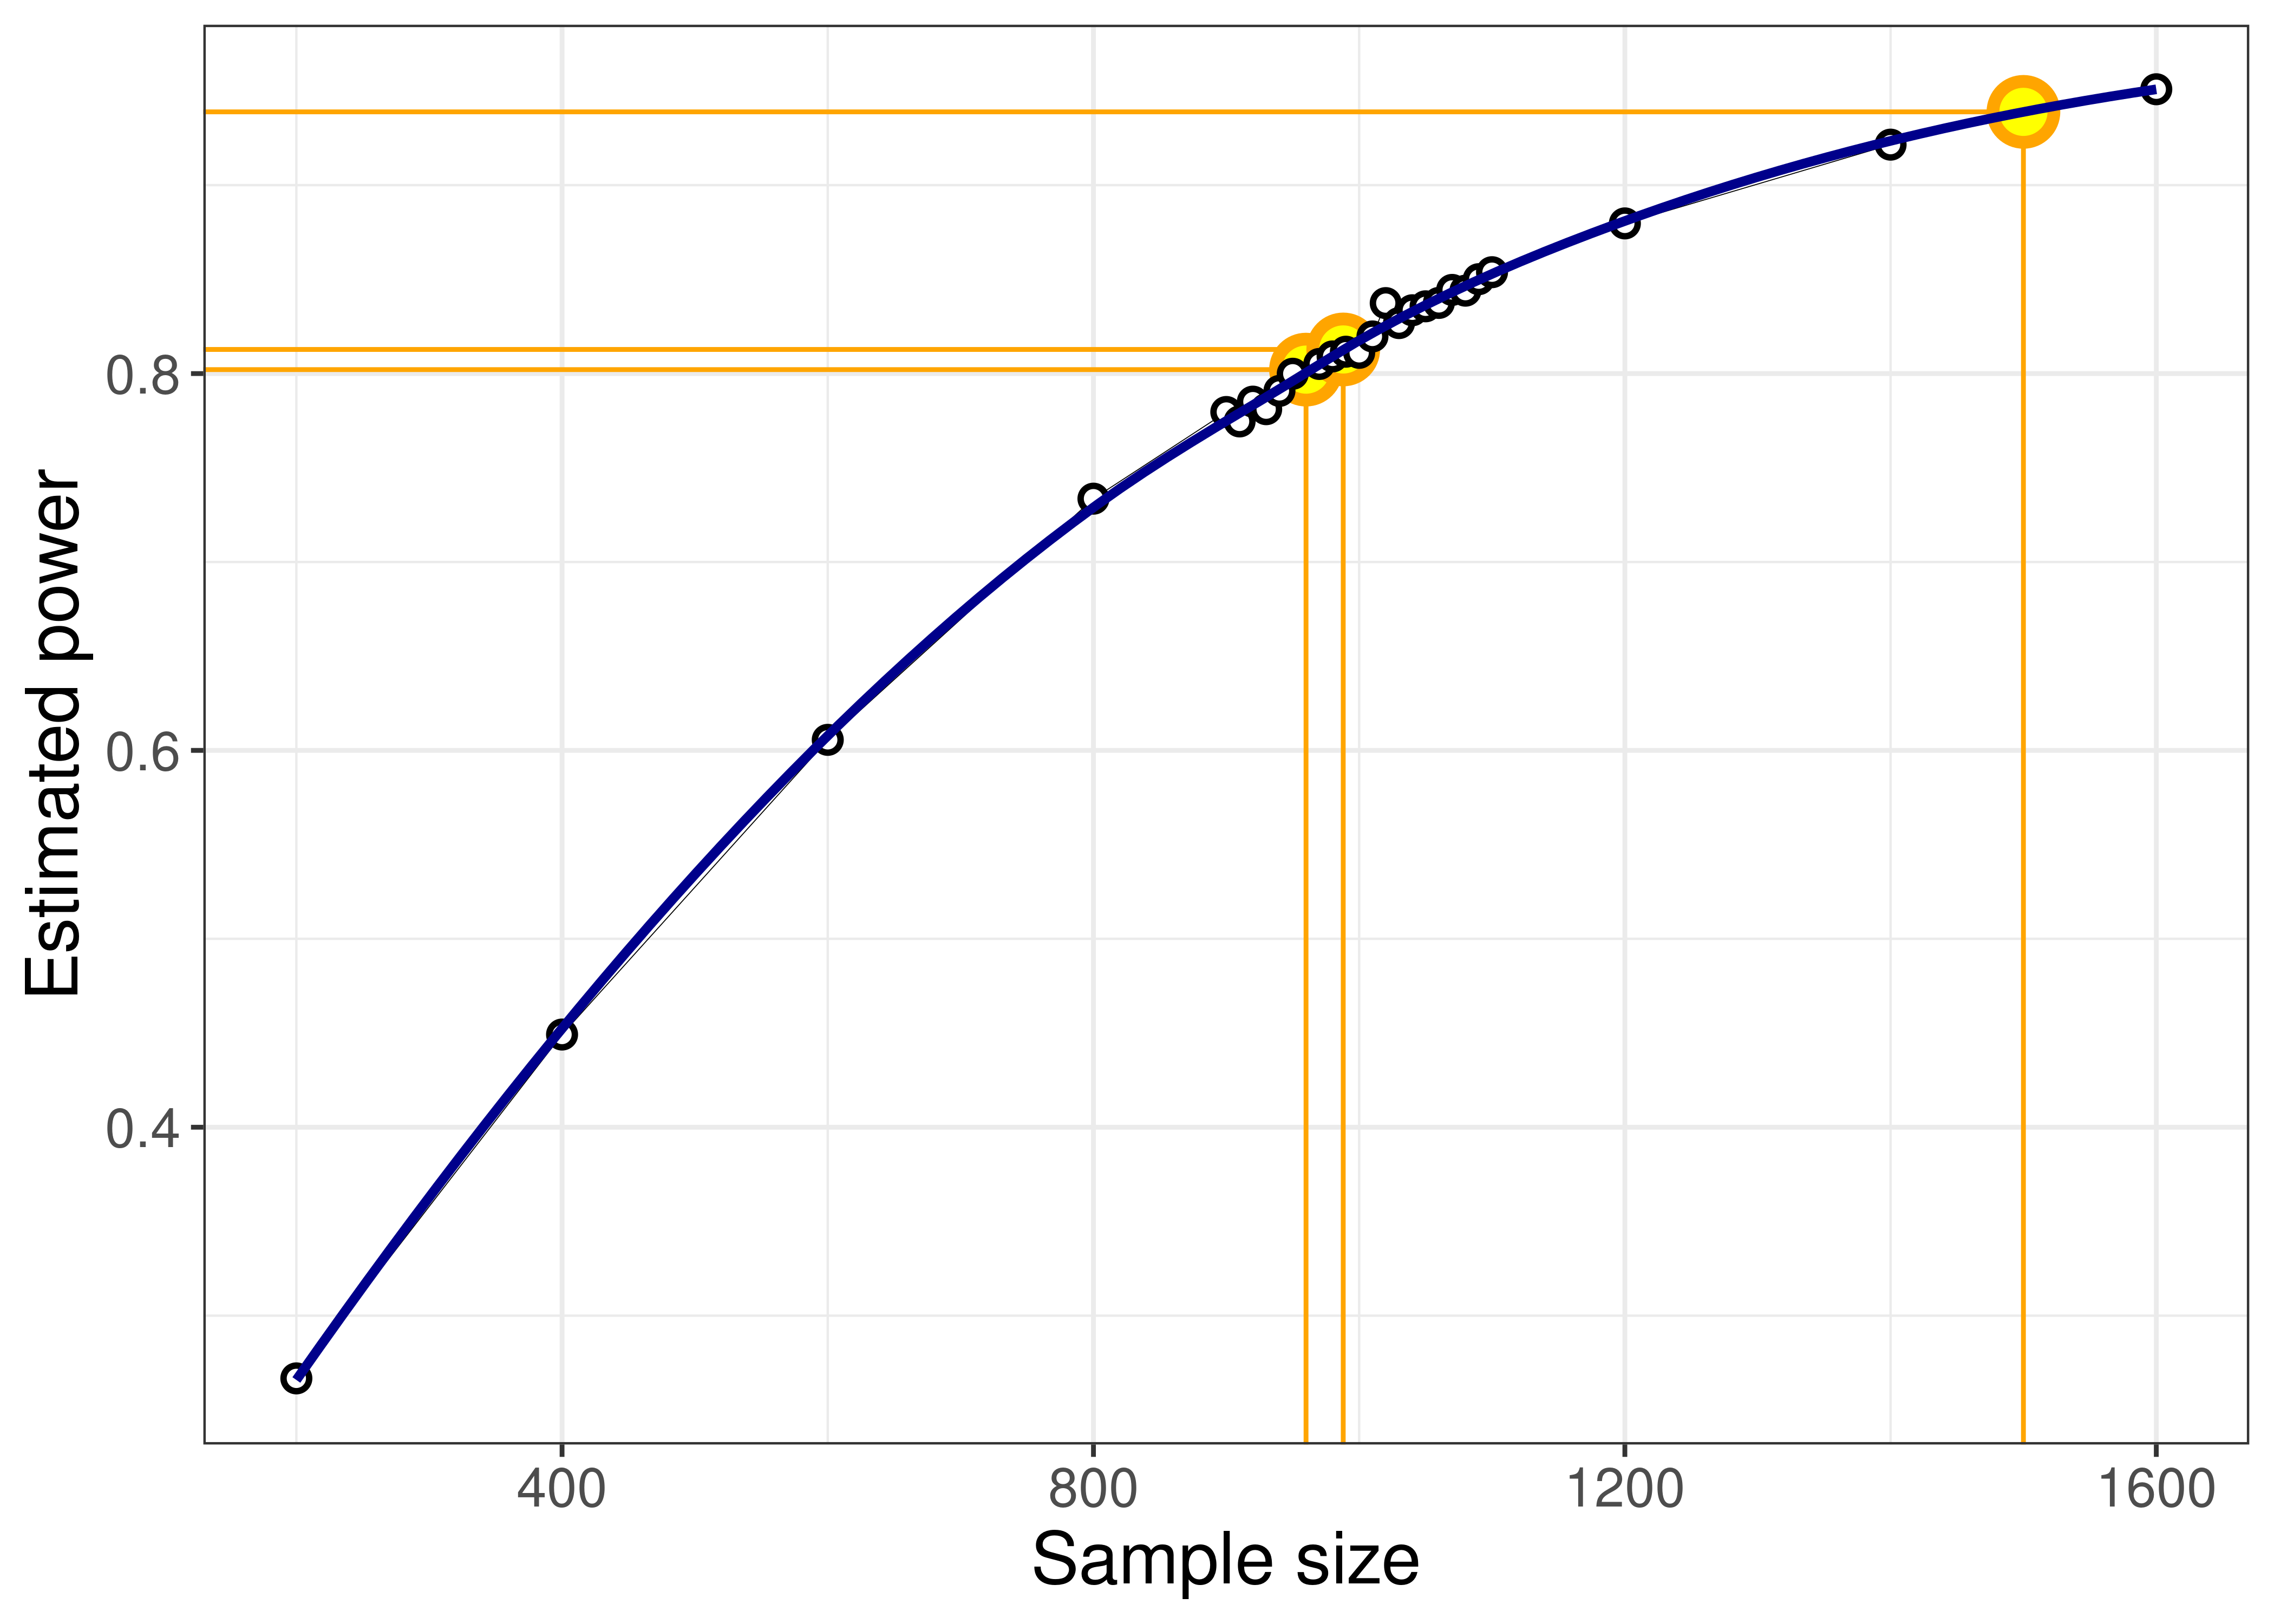
\includegraphics[width=.5\linewidth]{./../analysis/code/R/pipeline_files/figure-html/power-1.png}
    \caption{Estimated power for different sample sizes is obtained as the proportion of synthetic data sets in which the null hypothesis of no association between WMH volume and time spent in high-occupancy brain states an be rejected at the $\alpha=0.05$ significance level. Proportions are based on a total of \num{10000} synthetic data sets obtained by bootstrapping the data presented in \citep{Schlemm2022-he}. Highlighted in orange are the smallest sample size ensuring a power of at least \qty{80}{\percent} ($n=960$), the sample size of the pilot data ($n=988$, post-hoc power \qty{81.3}{\percent}), and the expected sample sample size for this replication study ($n=1500$, a-priori power \qty{93.9}{\percent}).}
    \label{fig:power}
\end{figure}

It is seen that a sample size of \num{960} would allow replication of the reported effect with a power of \qty{80.2}{\percent}.
We anticipate a sample size of \num{1500}, which yields a power of \qty{93.9}{\percent}.


\subsection{Multiverse analysis}
Both in \citep{Schlemm2022-he} and for our primary replication analysis we made certain analytical choices in the operationalisation of brain states and ischemic white matter disease, namely the use of the \textit{36p} confound regression strategy, the Schaefer-\num{400} parcellation and a BIANCA/LOCATE-based WMH segmentation algorithm.
The robustness of the association between WMH burden and time spent in high-occupancy states with regard to other choices will be explored in a multiverse analysis \citep{Steegen2016-ze}. Specifically, in an exploratory analysis, we will estimate brain states from BOLD time series processed according to a variety of established confound regression strategies and aggregated over different cortical brain parcellations (\Cref{tab:multiverse}, \cite{ciric2018mitigating,Ciric2017-cl}). Extent of cSVD will additionally be quantified by the volume of deep and periventricular white matter hyperintensities.

\renewcommand\cellset{\renewcommand\arraystretch{0.5}%
    \setlength\extrarowheight{0pt}}
\begin{table}[bt]
    \begin{threeparttable}
        \begin{subtable}[t]{.75\textwidth}
            \label{tab:parcellations2}
            % Use "S" column identifier to align on decimal point 
            \begin{tabularx}{\textwidth}{l l l}
                \toprule
                \textbf{Name of the atlas}  & \textbf{\#parcels}                                  & \textbf{Reference}          \\
                \midrule
                Desikan--Killiany           & \num{86}                                            & \cite{desikan2006automated} \\
                AAL                         & \num{116}                                           & \cite{tzourio2002automated} \\
                Harvard--Oxford             & \num{112}                                           & \cite{makris2006decreased}  \\
                glasser360                  & \num{360}                                           & \cite{Glasser2016-ia}       \\
                gordon333                   & \num{333}                                           & \cite{Gordon2016-wy}        \\
                power264                    & \num{264}                                           & \cite{Power2011-xf}         \\
                schaefer\{N\}               & \makecell[lt]{\num{100} \\ \num{200}\\ \num{400}}   & \cite{Schaefer2018-bo}      \\
                \bottomrule
            \end{tabularx}
            \begin{tablenotes}
                \item{AAL:} Automatic Anatomical Labelling
            \end{tablenotes}
            \caption{Parcellations}
        \end{subtable}
        \qquad
        \begin{subtable}[t]{.75\textwidth}
            \label{tab:parcellations}
            % Use "S" column identifier to align on decimal point 
            \begin{tabularx}{\textwidth}{l l l}
                \toprule
                \textbf{Design}        & \textbf{Reference}                 \\
                \midrule
                24p                    & \cite{friston1996movement}         \\
                24p + GSR              & \cite{macey2004method}             \\
                36p              & \cite{satterthwaite2013improved}   \\
                36p + spike regression & \cite{cox1996afni}                 \\
                36p + despiking        & \cite{satterthwaite2013improved}   \\
                36p + scrubbing  & \cite{power2014methods}            \\
                aCompCor               & \cite{muschelli2014reduction}      \\
                tCompCor               & \cite{behzadi2007component}        \\
                AROMA                  & \cite{pruim2015ica}                \\
                \bottomrule
            \end{tabularx}
            \begin{tablenotes}
                \item GSR: Global signal regression, AROMA: Automatic Removal of Motion Artifacts
            \end{tablenotes}
            \caption{Confound regression strategies, adapted from \citep{Ciric2017-cl}}
        \end{subtable}
        \makeatletter\def\TPT@hsize{}\makeatletter
    \end{threeparttable}
    \mycaption{Multiverse analysis}{Overview over different brain parcellations and confound regression strategies implemented using xcpEngine \citep{ciric2018mitigating}. A total of $9\times 9=81$ analytical combinations were explored to assess the robustness of our results with respect to these processing choices.}
    \label{tab:multiverse}
\end{table}

For each combination of analytical choice of confound regression strategy, parcellation and subdivision of white matter lesion load ($9\times9\times3=243$ scenarios in total) we will quantify the association between WMH load and average time spent in high-occupancy brain states using odds ratio and \qty{95}{\percent} confidence intervals as described above.

No hypothesis testing and will be carried out in these multiverse analyses. They rather serve to inform about the robustness of the outcome of the test of the primary hypothesis.
Any substantial conclusions about the association between severity of cerebral small pathology and time spent in high-occupancy brain states, as stated in the Scientific Question in \Cref{tab:SDT}, will be drawn from the primary analysis using pre-specified methodological choices.

\section{Further exploratory analysis}
In previous work, two high-occupancy brain states were related to the default-mode network \citep{Cornblath2020-fu}.
We will further explore this relation by computing, for each individual brain state, the cosine similarity of the positive and negative activations of the cluster’s centroid with a set of a-priori defined functional ‘communities’ or networks \citep{Schaefer2018-bo,Yeo2011-qg}.
Results will be thus visualized as spider plots for the Schaefer, Gordon and Power atlasses.

In further exploratory analyses we plan to describe the associations between brain state dynamics and other measures of cognitive ability, such as memory and language.
\section{Results}
For this replication study, a total of \num{2648} datasets were available, of which \num{970} were already included in our previous analysis and thus discarded. In \num{13} of the resulting \num{1678} datasets, one or more MRI sequences were missing. Of the complete datasets (n=\num{1665}), we excluded \num{5} participants due to intra-axial space-occupying lesions. An additional \num{9} participants were excluded because of unsuccessful preprocessing, WMH segmentation, or xcpEngine failure, resulting in \num{1651} datasets for analysis. A study-flowchart is provided in \Cref{fig:flowchart}.

\begin{figure}
    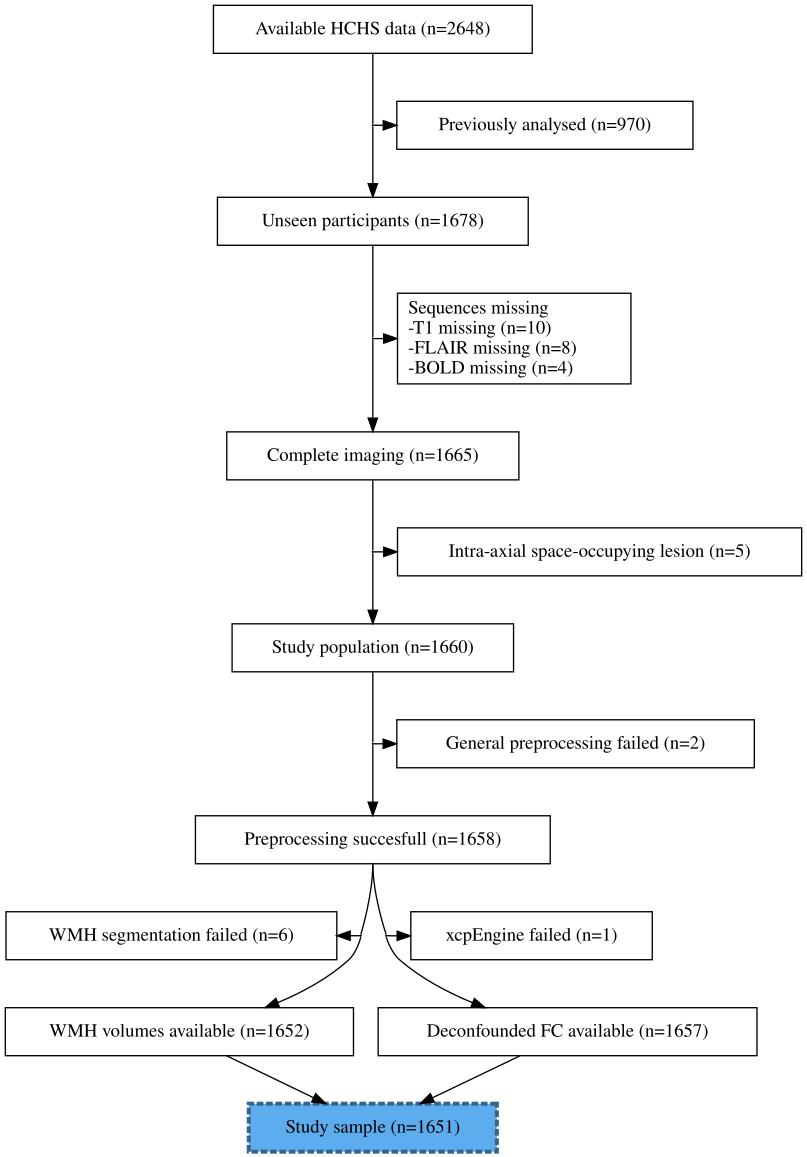
\includegraphics[width=0.5\linewidth]{./../analysis/code/R/FLOW.png}
    \mycaption{Study flowchart}{Composition of the study population after application of inclusion and exclusion criteria, and image processing.}
    \label{fig:flowchart}
\end{figure}




%\addtocounter{table}{-1}
\begin{table}
\centering
\setlength{\LTpost}{0mm}
\begin{longtable}{ll}
\toprule
 & \textbf{N = 1,651} \\ 
\midrule
\emph{Demographics} (no Missing n (\%))\\
\hline
Age, \unit{\year} &  \\ 
\quad Median (IQR) & 66 (59 -- 72) \\ 
Sex &  \\ 
\quad Male & 940/1651 (57\%) \\ 
\quad Female & 711/1651 (43\%) \\ 
\rule{0pt}{3ex}    
\emph{Cardiovascular risk factors}\\
\hline
Hypertension & \\
\quad Present & 1177/1611 (73.1\%) \\
\quad Missing n (\%) & 85 (5.1\%) \\
Diabetes & \\
\quad Present & 157/1566 (10\%)\\
\quad Missing n (\%) & 40 (2.4\%) \\
Smoking & \\ 
\quad Present & 200/1360 (14.7\%) \\
\quad Missing n (\%) & 201 (12.9\%\%)\\
Hyperlipidaemia & \\
\quad Present & 426/1578 (27\%)\\
\quad Missing n (\%) & 73 (4.4\%) \\
\rule{0pt}{3ex}    
\emph{Cognitive test results}\\
\hline
MMSE, \# (max. 30) &  \\ 
\quad Median (IQR) & 28 (27 -- 29) \\ 
\quad Missing n (\%) & 129 (7.8\%) \\ 
Vocabulary (MWT-B), \# (max. 37) &  \\ 
\quad Median (IQR) & 32 (30 -- 34) \\ 
\quad Missing n (\%) & 295 (18\%) \\ 
Word recall, \# (max. 10) &  \\ 
\quad Median (IQR) & 8 (6 -- 9) \\ 
\quad Missing n (\%) & 180 (11\%) \\ 
Animal Naming &  \\ 
\quad Median (IQR) & 24 (20 -- 29) \\ 
\quad Missing n (\%) & 116 (7.0\%) \\ 
TMT-A, seconds &  \\ 
\quad Median (IQR) & 38 (31 -- 48) \\ 
\quad Missing n (\%) & 144 (8.7\%) \\ 
TMT-B, seconds &  \\ 
\quad Median (IQR) & 83 (65 -- 110) \\ 
\quad Missing n (\%) & 162 (9.8\%) \\ 
\rule{0pt}{3ex}    
\emph{History}\\
\hline
Diagnosed dementia & \\
\quad Present & 6/1645 (0.4\%)\\
\quad Missing n (\%) & 6 (0.4\%) \\
Years of education &  \\ 
\quad Median (IQR) & 13 (12 -- 16) \\ 
\quad Missing n (\%) & 34 (2\%) \\ 
\bottomrule
\end{longtable}
\addtocounter{table}{-1}
\mycaption{Descriptive statistics of the study population}{Data are presented as median (interquartile range) or count (percentage) of non-missing items, as appropriate. Number of percentage of missing items are reported separately.}
\label{tab:democog}
\end{table}


Baseline demographic and cognitive values, including the number of missing items, are reported in \Cref{tab:democog}.

WMH volumes (median \qty{1.05}{\milli\litre}, IQR \qtyrange{0.47}{2.37}{\milli\litre}), motion estimates, and fractional occupancies of brain states 1 through 5 are reported in \Cref{tab:fracocc}. 
%\addtocounter{table}{-1}
\begin{table}
\centering
\setlength{\LTpost}{0mm}
\begin{longtable}{ll}
\toprule
& \textbf{N = 1,651} \\ 
\midrule
WMH volume\textsuperscript{1}, \unit{\milli\litre} & \\
\quad Total & 1.05 (0.47 -- 2.37), 9\,Z\\
\quad Periventricular & 0.94 (0.43 -- 2.04), 9\,Z \\
\quad Deep & 0.10 (0.03 -- 0.37), 344\,Z  \\
Motion during rs-fMRI \\
\quad Framewise displacement, \unit{\milli\metre} & 0.21 (0.15 -- 0.63)\\
\quad RMSD, \unit{\milli\metre} & 0.086 (0.058 -- 0.12)\\
\quad DVARS &  27.8 (24.3 -- 31.8)\\
Fractional occupancy, \% \\
\quad DMN+ & 24.8 (20.8 -- 28.0) \\ 
\quad DMN- & 24.0 (20.0 -- 28.0) \\ 
\quad S3 & 18.4 (15.2 -- 22.4) \\ 
\quad S4 & 16.8 (12.8 -- 20.8) \\ 
\quad S5 & 15.2 (12.0 -- 19.2) \\
\bottomrule
\end{longtable}
\addtocounter{table}{-1}
\textsuperscript{1}Number of zero values indicated by Z
\mycaption{Structural and functional imaging characteristics}{Data are presented as median (interquartile range). Supratentorial WMH volumes were obtained by semiautomatic segmentation of FLAIR images using a BINACA/LOCATE-based $k$-nearest neighbours algorithm and stratified by their distance to the lateral ventricles (<\qty{10}{\milli\metre}, periventricular; >\qty{10}{\milli\metre}, deep). Motion parameters were estimated during fMRIprep processing of BOLD scans. Fractional occupancies were calculated by assigning individual BOLD volumes to one of five discrete brain states defined by k-means clustering-based co-activation pattern analysis.Two high-occupancy states are labelled DMN+ and DMN- in view of their network connectivity profiles as shown in \Cref{fig:spider}.}
\label{tab:fracocc}
\end{table}


In an outcome-neutral quality check of the implementation of (i) the MRI processing pipeline, (ii) brain state estimation, and (iii) co-activation pattern analysis, the mean difference in fractional occupancy between high- and low-occupancy states was consistently maintained, with a point-estimate of the separation between two high-occupancy and three low-occupancy states of \qty{6.7}{\percent} (\qty{95}{\percent} confidence interval, \qtyrange{6.2}{7.1}{\percent}) in the \emph{36p} paradigm. 
This indicates that the implementation of the pipeline was correct and that the brain state estimation and co-activation pattern analysis worked as intended. 


\subsection{Pre-registered hypotheses}
\subsubsection{Association between WMH load and fractional occupancy}
The results of the test of our primary preregistered hypothesis of an association between supratentorial WMH volume and the time spent in high-occupancy brain states are shown in \Cref{fig:hyp1} and \Cref{tab:hyp1}.

\begin{figure}
    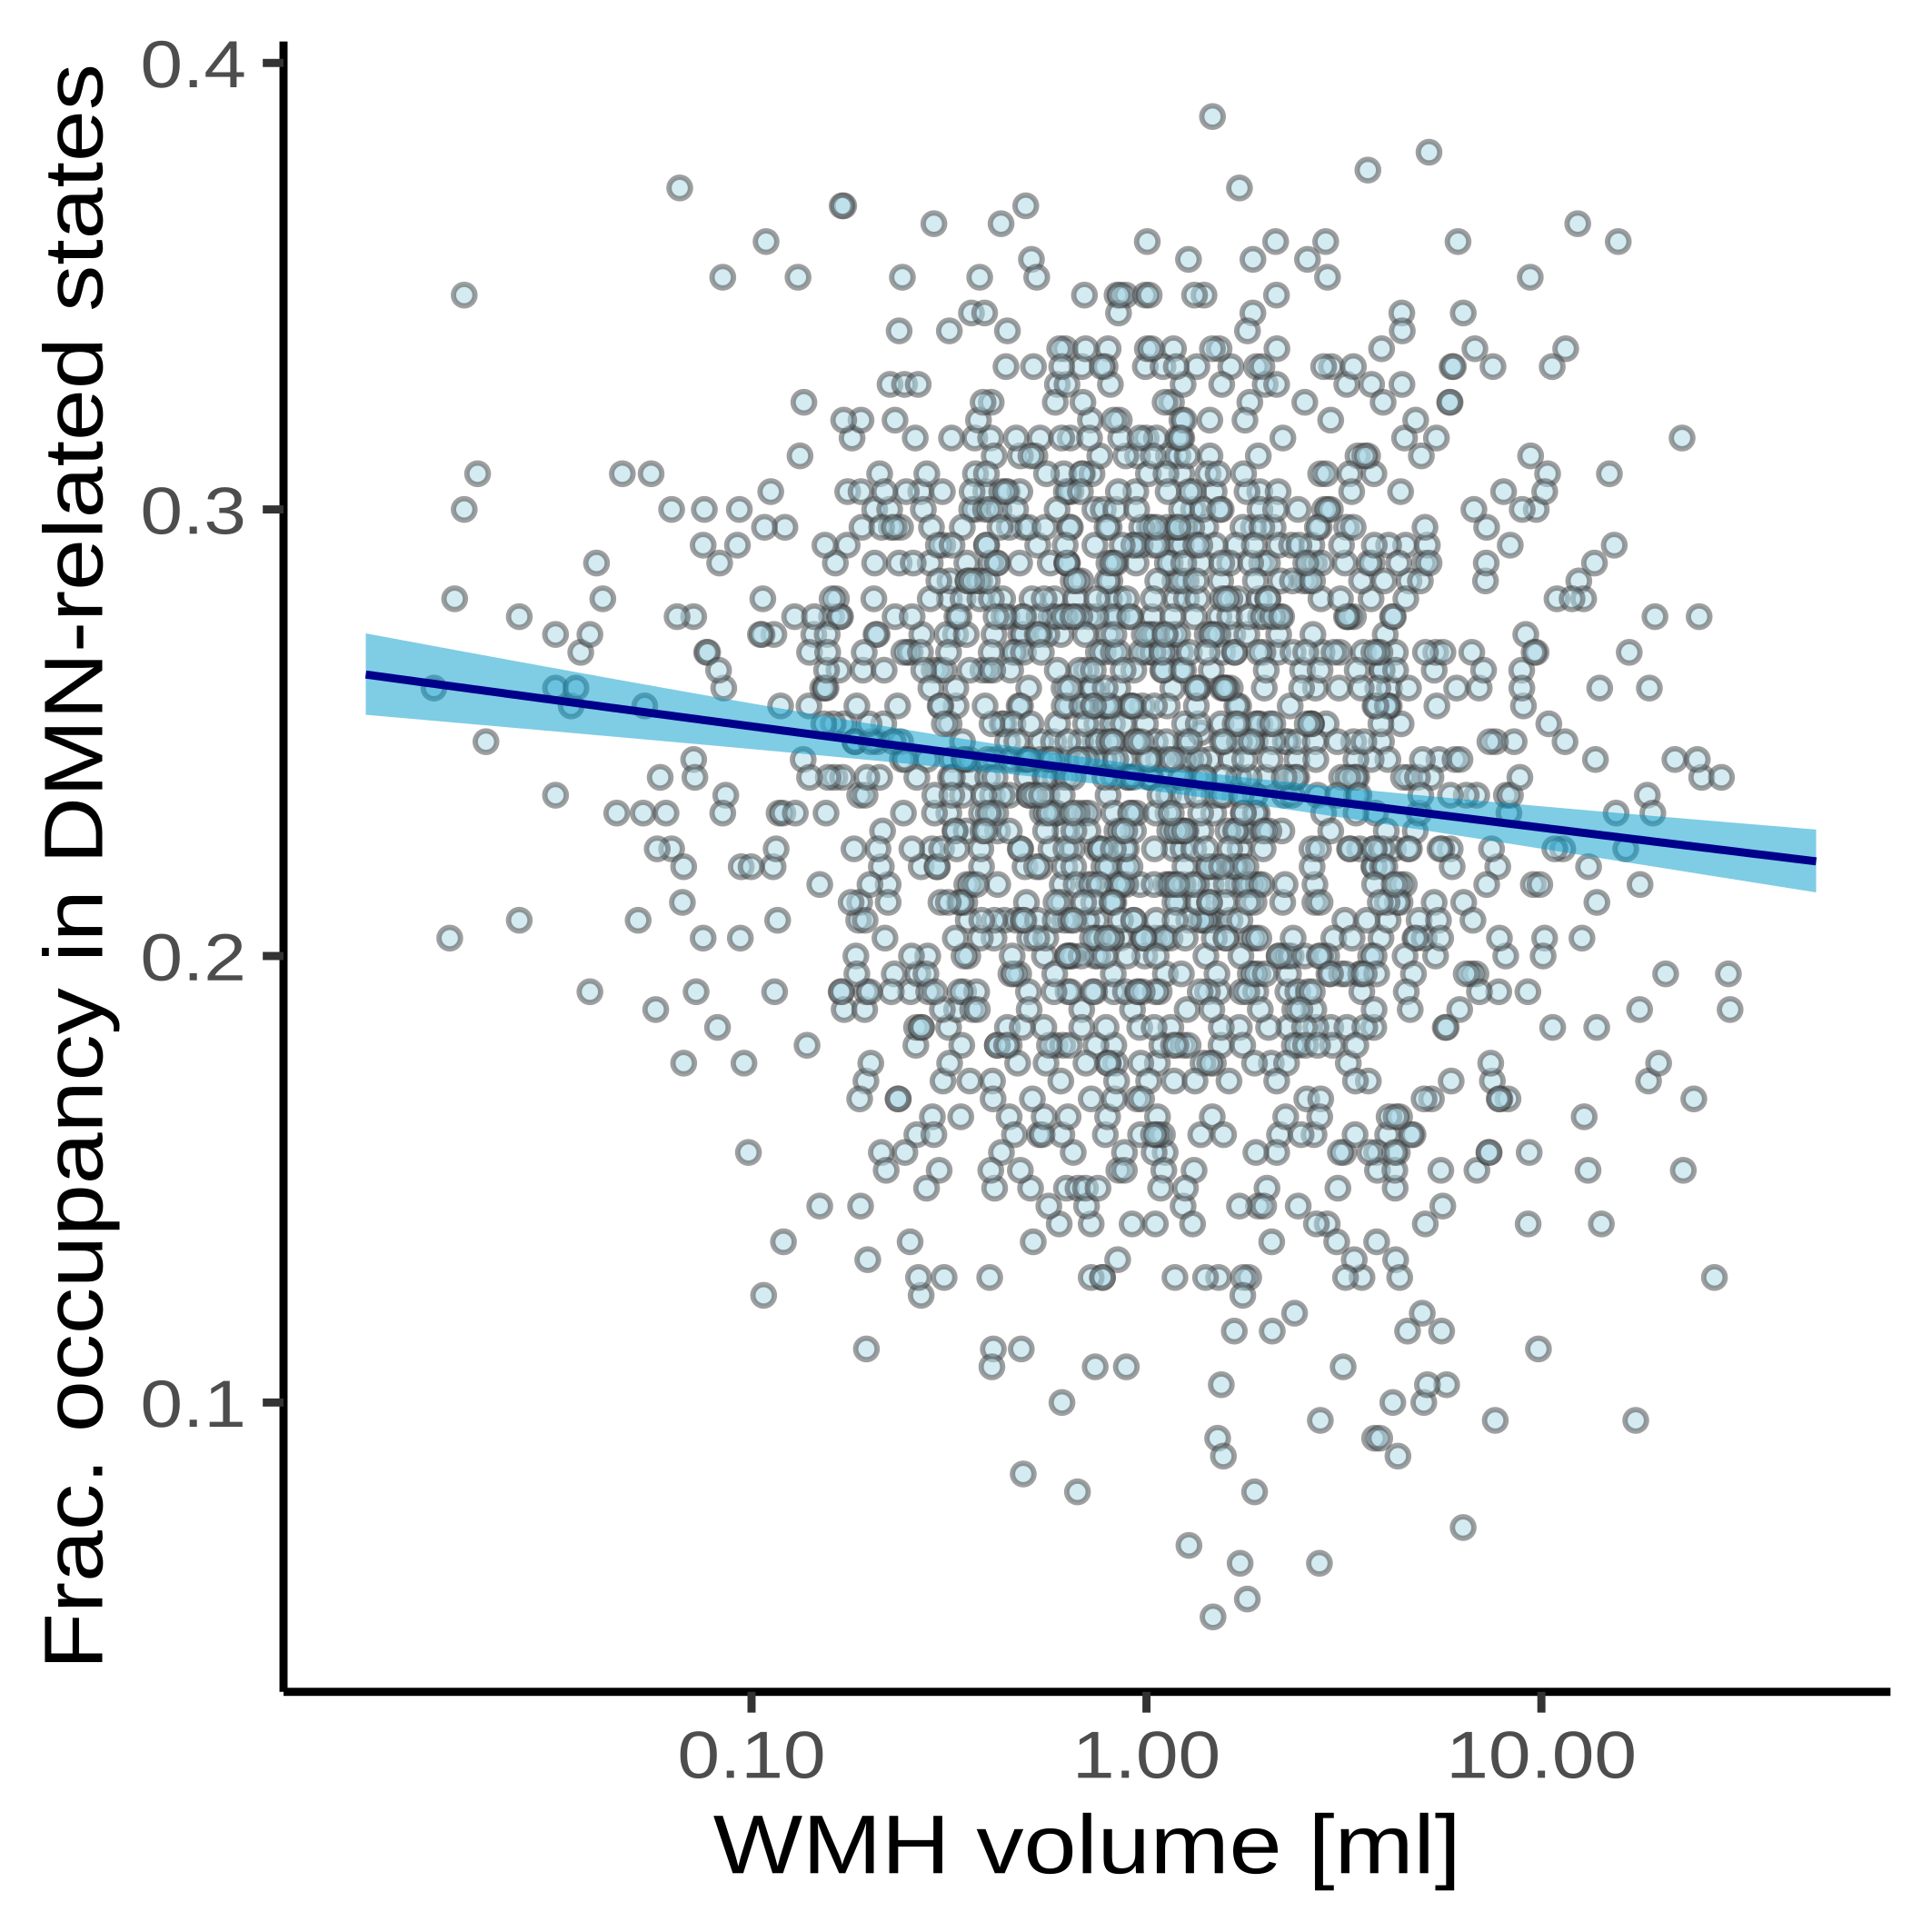
\includegraphics[width=.5\linewidth]{./../analysis/derivatives/Figures/Fig_hyp1.png}
    \mycaption{Association between time spent in high-occupancy brain states and supratentorial WMH volume}{Point estimates (black line) and 95\%-confidence region (light blue ribbon) of the conditional mean fractional occupancy are obtained from unadjusted beta regression modelling. Each marker represents one of N=1642 independent participants with a non-zero total WMH volume. }
    \label{fig:hyp1}
\end{figure}

%\addtocounter{table}{-1}
\begin{table}
\centering
\setlength{\LTpost}{0mm}
\begin{longtable}{lccc}
\toprule
 & Estimate & P & 95\%-CI \\ 
\midrule
Intercept & 0.24 & <0.0001 & 0.21 -- 0.27 \\ 
WMH, per 5.1-fold increase\textsuperscript{1} & 0.94 & <0.0001 & 0.92 -- 0.96 \\ 
Age, per 10 years & 1.04 & 0.001 & 1.01 -- 1.06 \\ 
Female sex & 1.12 & <0.0001 & 1.09 -- 1.16 \\ 
$\mathbf{1}_{\{\operatorname{WMH=0}\}}$ & 0.93 & 0.477 & 0.75 -- 1.14 \\ 
\bottomrule
\end{longtable}
\textsuperscript{1} Interquartile ratio $2.37/0.468=5.06$
\mycaption{Association between time-spent in high-occupancy DMN-related brain states and WMH volume adjusted for age and sex}{Beta regression table estimated from $n=1651$ independent participants using the model equation $\operatorname{FO}^{\text{high}} \sim \log{\operatorname{WMH}^+} + \mathbf{1}_{\{\operatorname{WMH=0}\}} + \operatorname{age} + \operatorname{sex}$.}
\label{tab:hyp1}
\end{table}


Adjusted for age and sex, there was a \num{0.94}-fold reduction in the odds of occupying a high-occupancy brain state for every \num{5.1}-fold increase in WMH load (P \num{5.01e-8}).

\subsubsection{Association between executive function and fractional occupancy in DMN-related states}

The results of the test of our secondary preregistered hypothesis of an association between time spent in high-occupancy brain states and executive function as measured by the complete part B of the TMT are shown in \Cref{fig:hyp2} and \Cref{tab:hyp2}.

\begin{figure}
    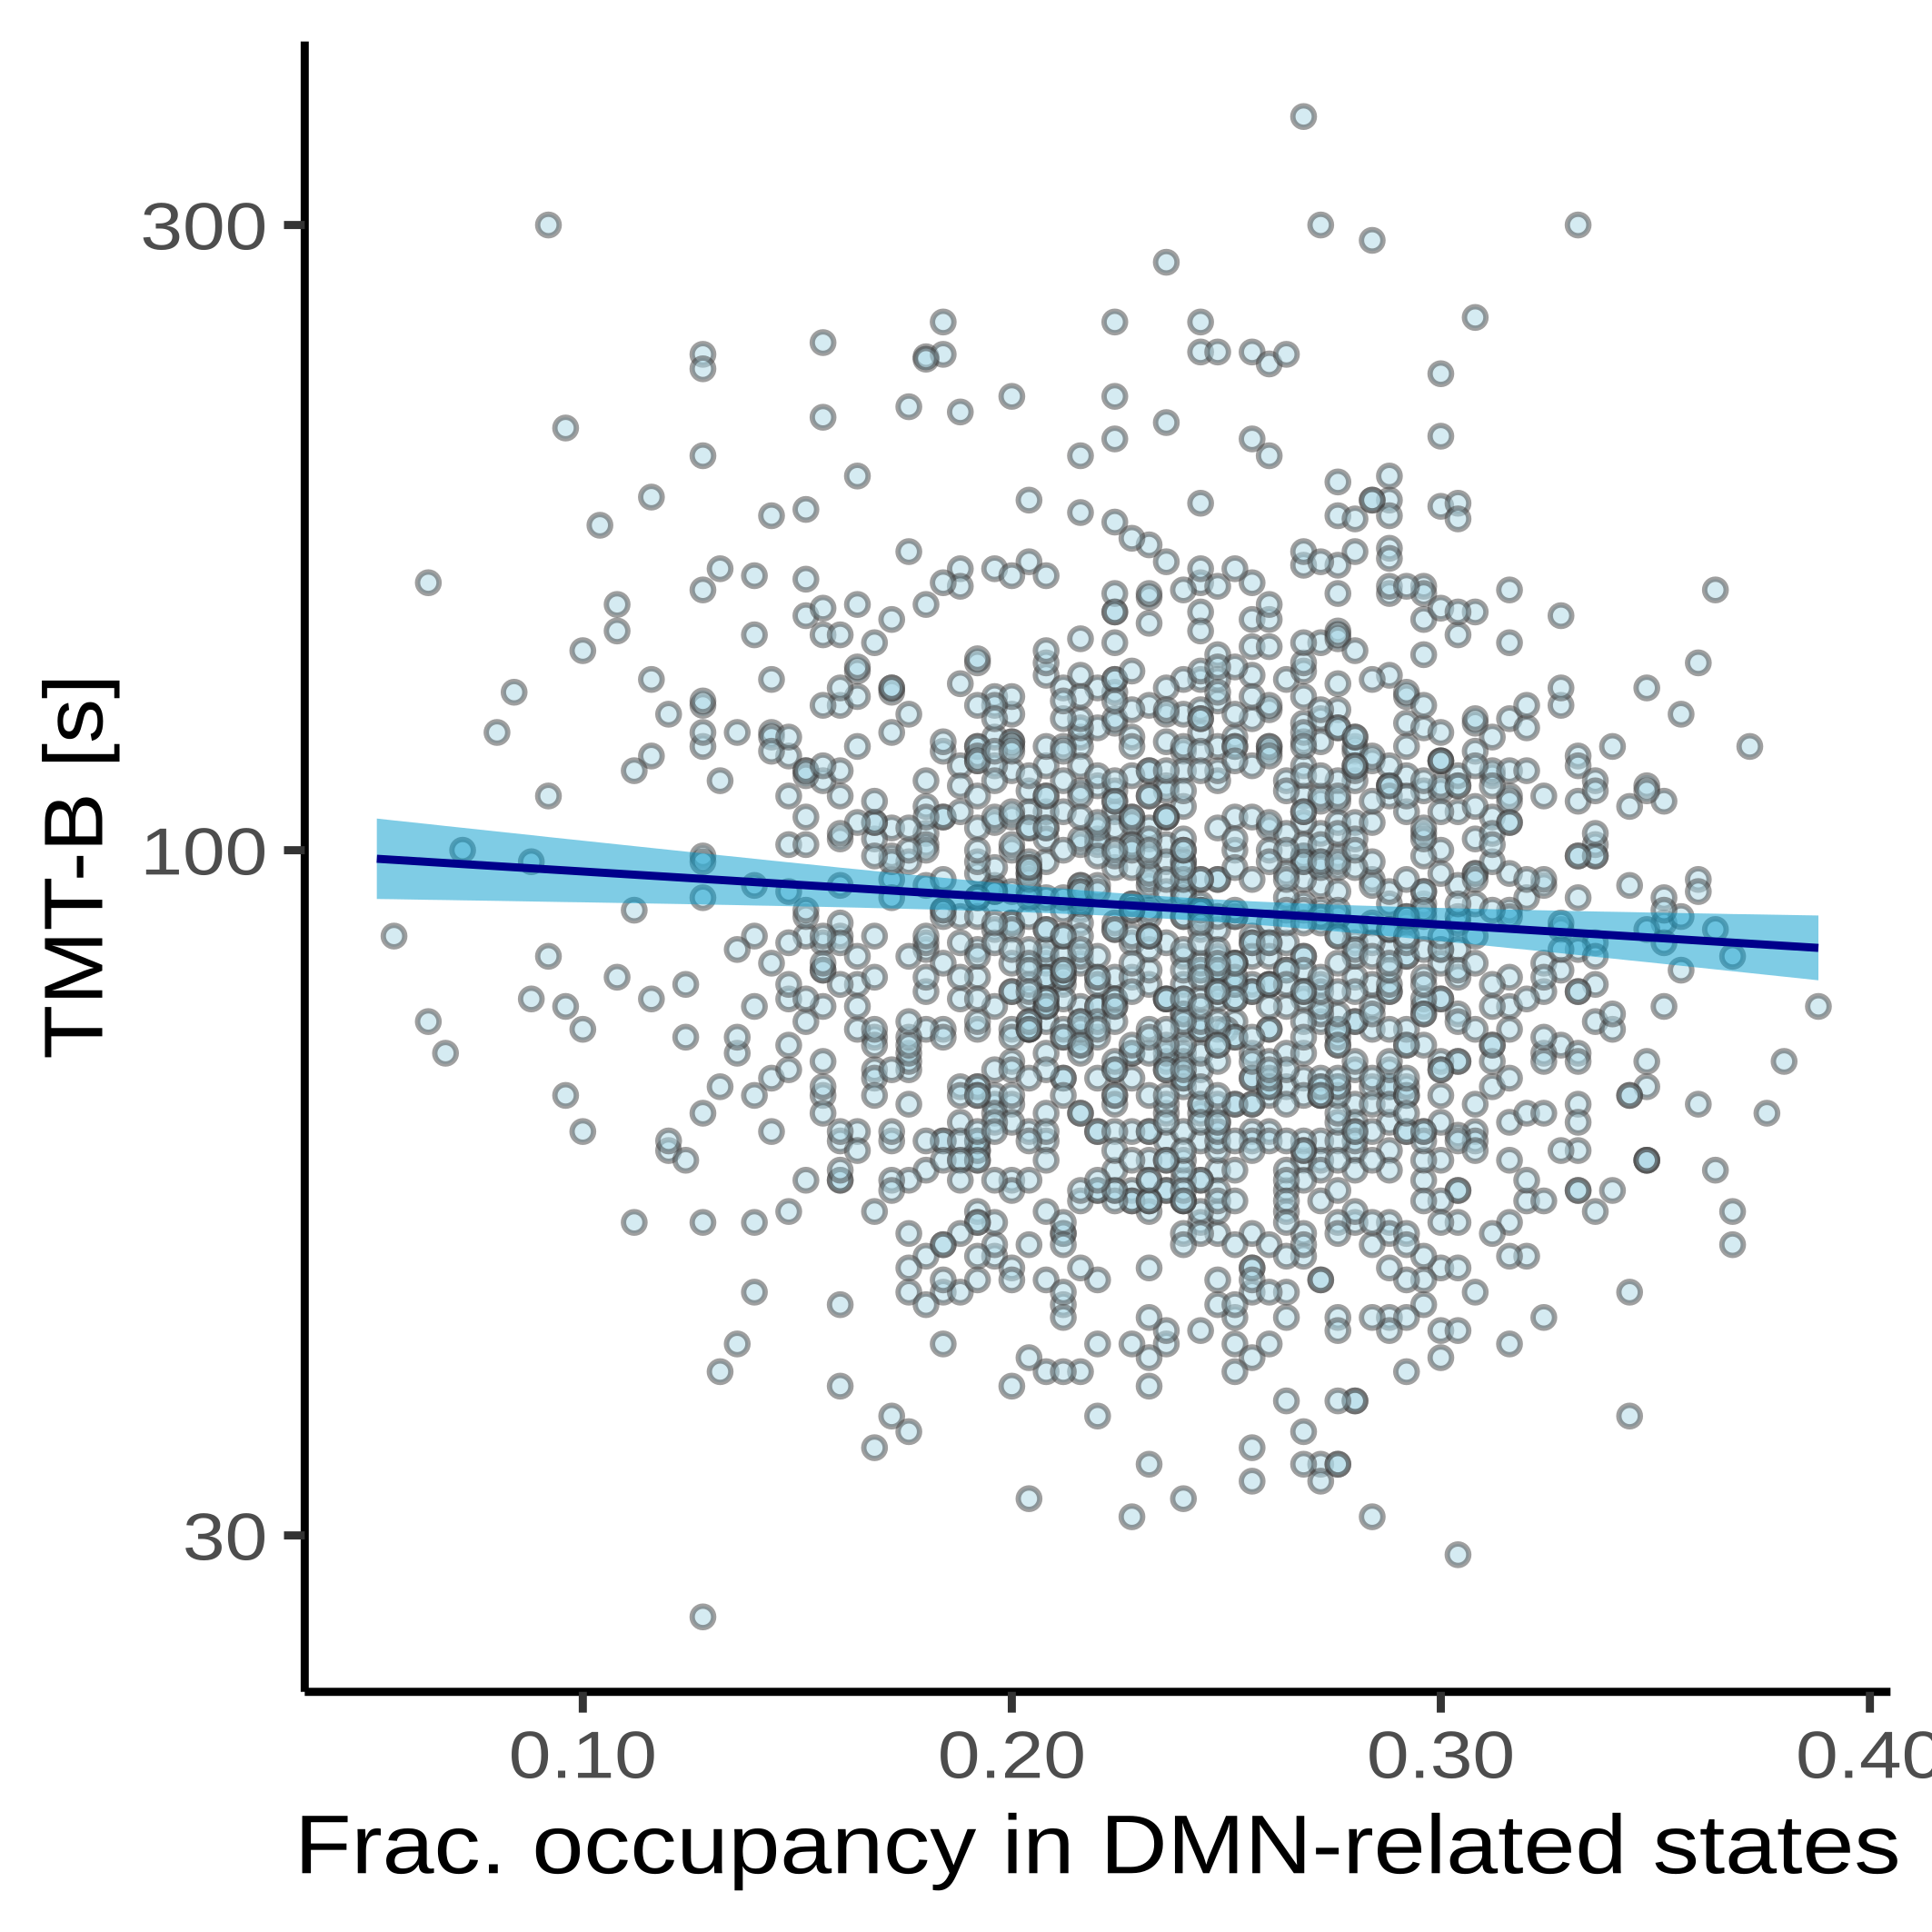
\includegraphics[width=.5\linewidth]{./../analysis/derivatives/Figures/Fig_hyp2.png}
    \mycaption{Association between time spent in high-occupancy DMN-related brain states and TMT-B completion time}{Point estimates (black line) and 95\%-confidence region (light blue ribbon) of the conditional mean TMT-B completion time are obtained from unadjusted Gamma regression modelling. Each marker represent one of N=1482 independent participants with non-zero total WMH volume and available TMT-B data.}
    \label{fig:hyp2}
\end{figure}

\begin{table}
\setlength{\LTpost}{0mm}
\begin{longtable}{lccc}
\toprule
 & Estimate & P & 95\%-CI \\ 
\midrule
Intercept & 53.41 & $<0.0001$ & 42.7 -- 66.8 \\ 
$\operatorname{FO}^{\text{high}}$, per 5\% & 0.98 & 0.0116 & 0.96 -- 0.99 \\ 
WMH, per 5.1-fold increase\textsuperscript{1} & 1.01 & 0.367 & 0.98 -- 1.05 \\ 
Age, per 10 years & 1.18 & <0.0001 & 1.15 -- 1.21 \\ 
Female sex & 0.99 & 0.666 & 0.95 -- 1.03 \\ 
Education, per year & 0.97 & <0.0001 & 0.97 -- 0.98 \\ 
$\mathbf{1}_{\{\operatorname{WMH=0}\}}$ & 0.97 & 0.398 & 0.92 -- 1.03 \\
\bottomrule
\end{longtable}
\addtocounter{table}{-1}
\textsuperscript{1} Interquartile ratio $2.37/0.468=5.06$
\mycaption{Association between TMT-B and time spent in high-occupancy DMN-related brain states adjusted for age, sex, WMH volume and years of education}{Gamma regression table estimated from $n=1483$ independent participants using the model equation $\operatorname{TMT-B} \sim \operatorname{FO}^{\text{high}} + \log{\operatorname{WMH}^+} + \mathbf{1}_{\{\operatorname{WMH=0}\}} + \operatorname{age} + \operatorname{sex}$.}
\label{tab:hyp2}
\end{table}

Adjusted for age, sex, WMH volume, and years of education, there was a \num{0.98}-fold reduction in the time to complete the TMT-B for every \qty{5}{\percent} increase in the time spent in high-occupancy brain states (P \num{0.0116}).


\subsection{Multiverse analysis}

In a multiverse analysis, the main findings of associations between WMH load and FO and, to a lesser extent, between FO and TMT-B were robust with respect to the processing choices of brain parcellation and confound regression strategy.

A nominally statistically significant negative association between the total WMH load and time spent in high-occupancy states was observed in 48/81 scenarios, with 8/81 significant positive associations occurring with the Desikan--Killiany parcellation only (\Cref{fig:mv}{A}). 
For periventricular (deep) WMH volume, the results were similarly robust with 49/81 (39/81) negative and 8/81 (0/81) positive associations of nominal statistical significance, respectively.

The secondary finding of an association between greater TMT-B times and lower fractional occupancy was less robust with only 16/81 nominally statistically significant negative and no significant positive associations, irrespective of operationalization of cSVD (total vs. periventricular vs. deep WMH volume) (\Cref{fig:mv}{B}).

\begin{figure}
    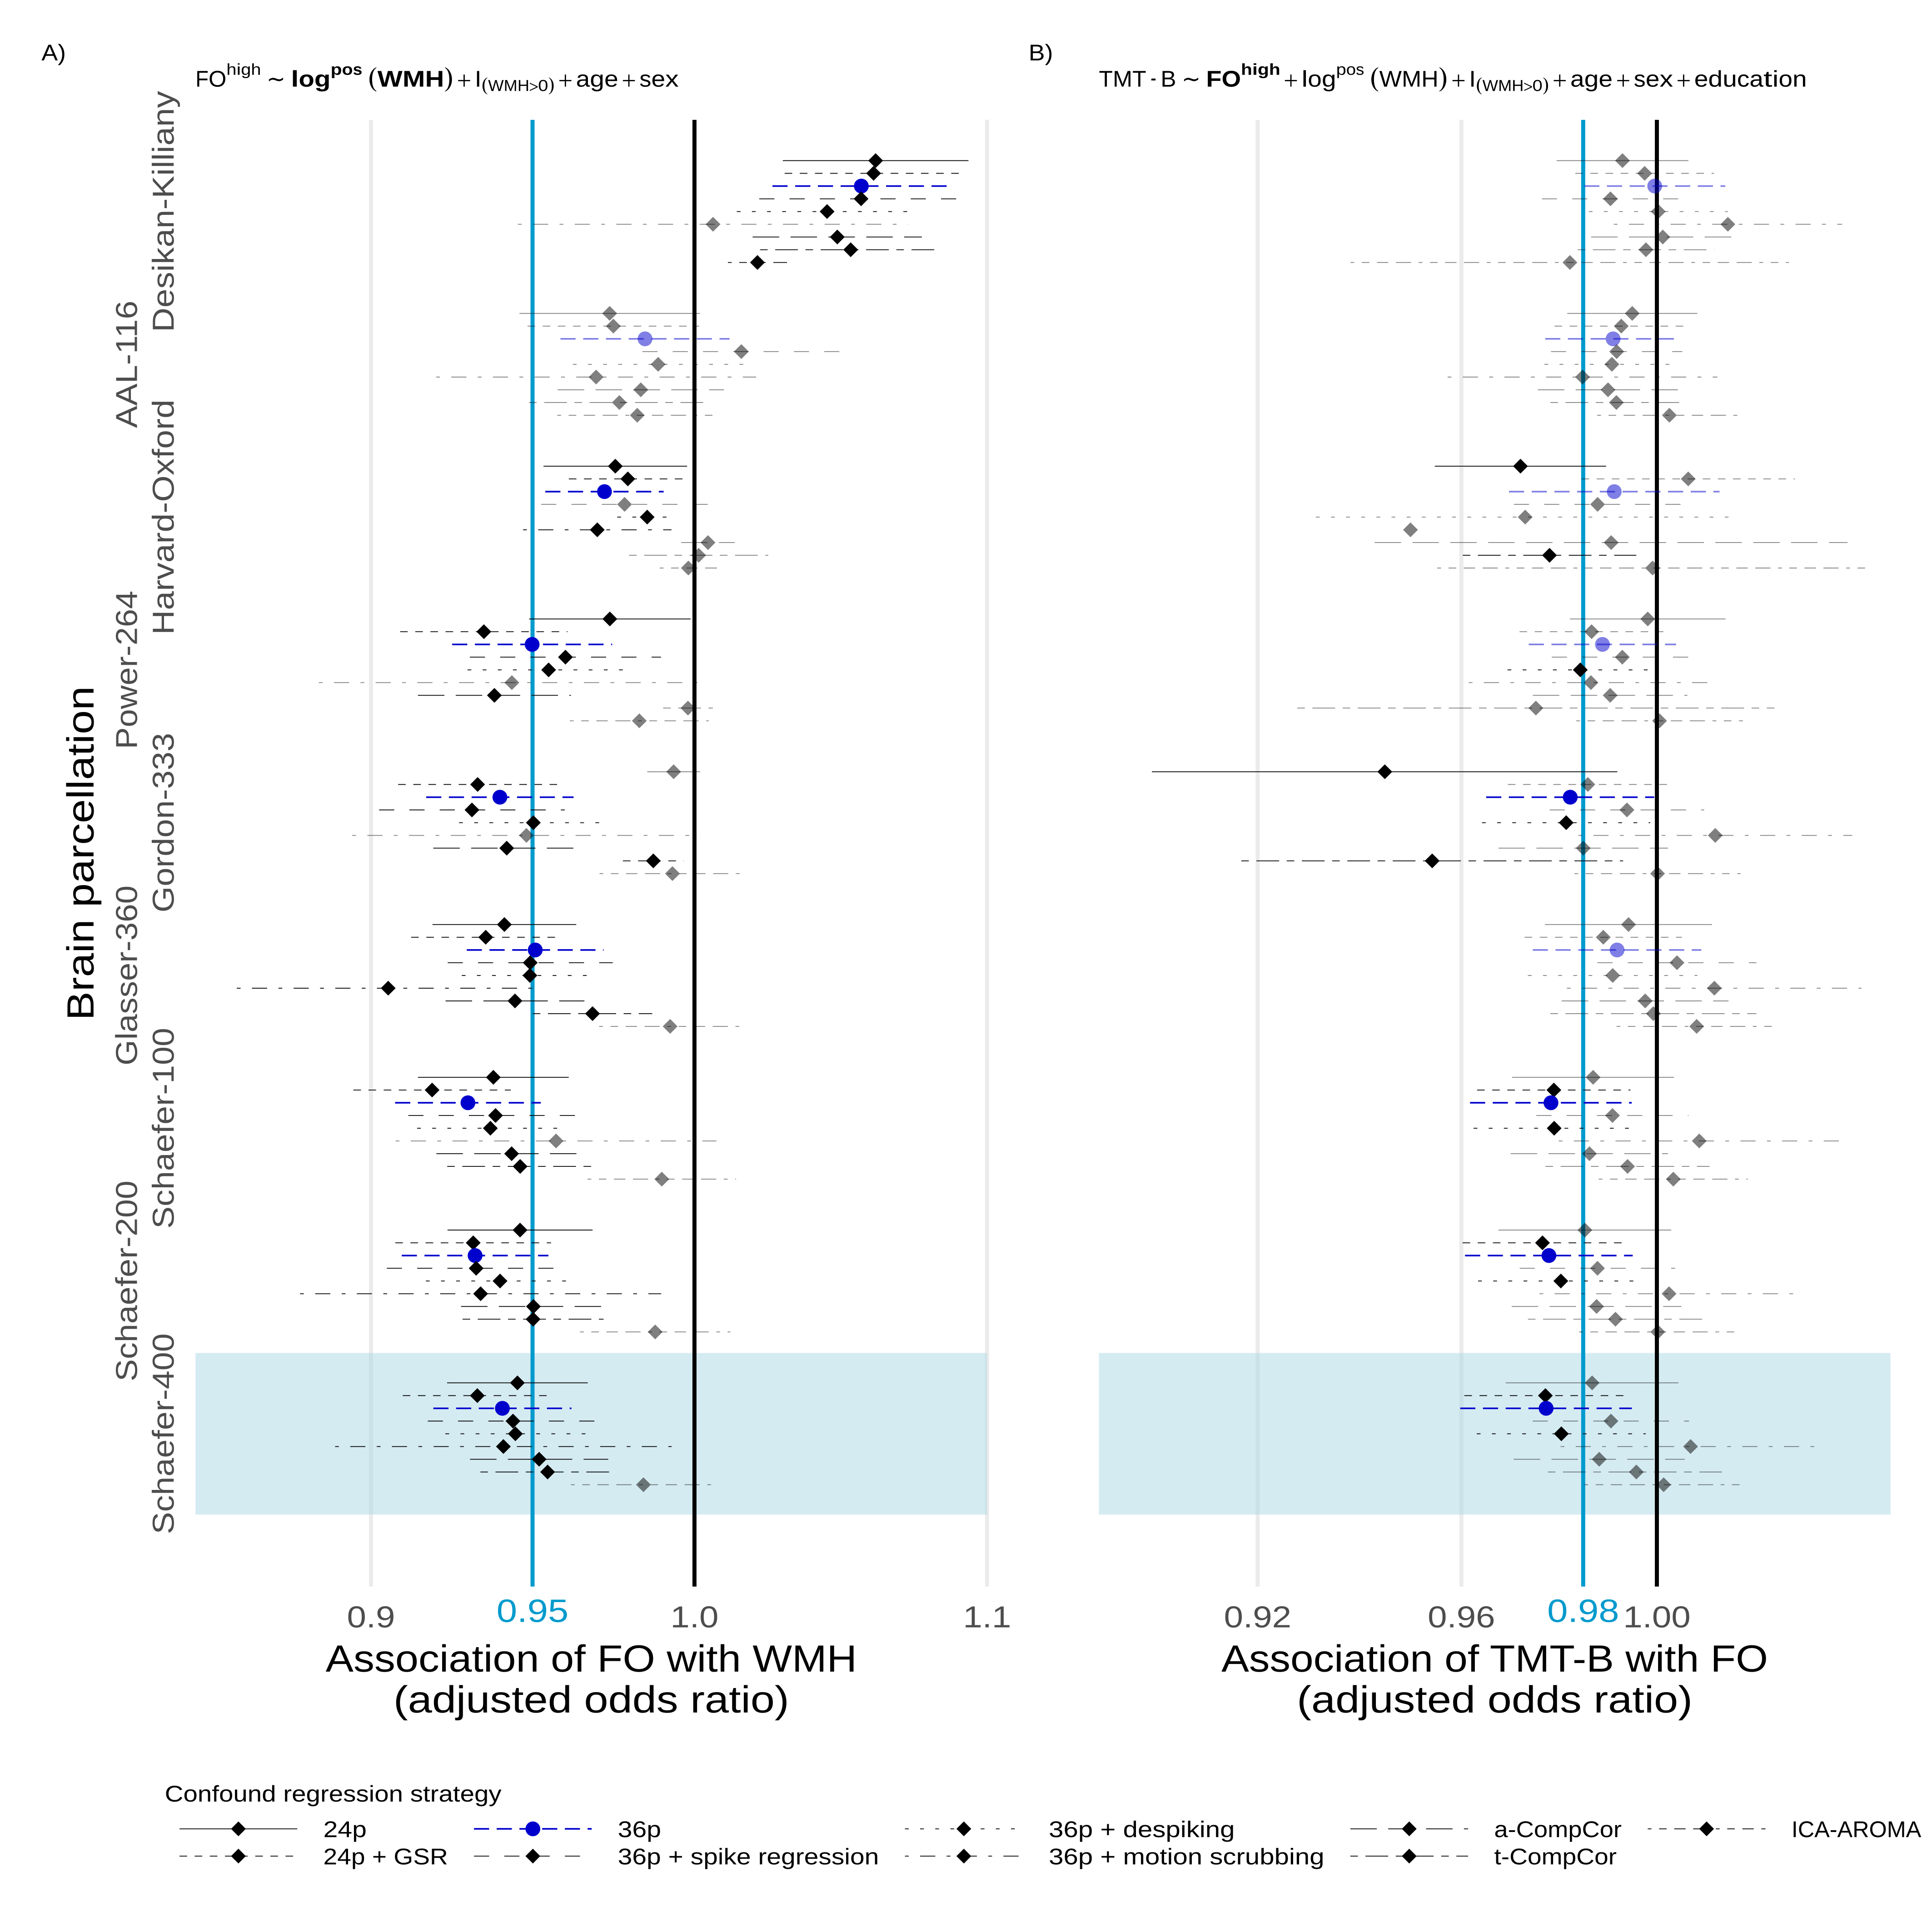
\includegraphics[width=\linewidth]{./../analysis/derivatives/Figures/Fig_mv.png}
    \mycaption{Multiverse analysis}{Adjusted effect size estimates of the associations between cSVD severity (WMH volume) and network dedifferentiation (less time spent in high-occupancy DMN-related brain states) [\textbf{A)}], and between network dedifferentiation and executive function (TMT-B completion time) [\textbf{B)}]. Effect sizes are given per 5.1-fold increase in WMH volume and a 5\%-increase in fractional occupancy, respectively. Markers and line segments indicate point estimates and 95\%-confidence intervals for adjusted odds ratios for different combinations of confound regression strategy and brain parcellation. The primary analytical choices are indicated by dark blue circles (\emph{}36p) and light blue shading (Schaefer-400). Model equations for beta and gamma regressions, respectively, are given at the top. Vertical lines indicate no effect (black) and the effect size observed in the discovery cohort \citep{Schlemm2022-he} (light blue), respectively, for reference. Effect sizes not reaching nominal statistical significance ($\alpha=0.05$) are shown desaturated. Corresponding data based on periventricular and deep WMH volumes are presented in the Supplementary Appendix.}
    \label{fig:mv}
\end{figure}

\subsection{Additional analyses}
\subsubsection{Connectivity profiles of brain states -- relation to default mode network}
Based on the cosine similarity between positive and negative activations of cluster centroids and indicator vectors of pre-defined large scale brain networks, network activation profiles were computed for brain states estimated from Schaefer parcellations of varying spatial resolutions.

\Cref{fig:spider} shows the corresponding spider plots, identifying states characterized by activation (DMN+) or suppression (DMN-) of the default mode network as states with the highest fractional occupancy.

\begin{figure}
    %\begin{subfigure}{1.0\textwidth}
    \includegraphics[width=\linewidth]{./../analysis/derivatives/Figures/surface/surfaces.png}
    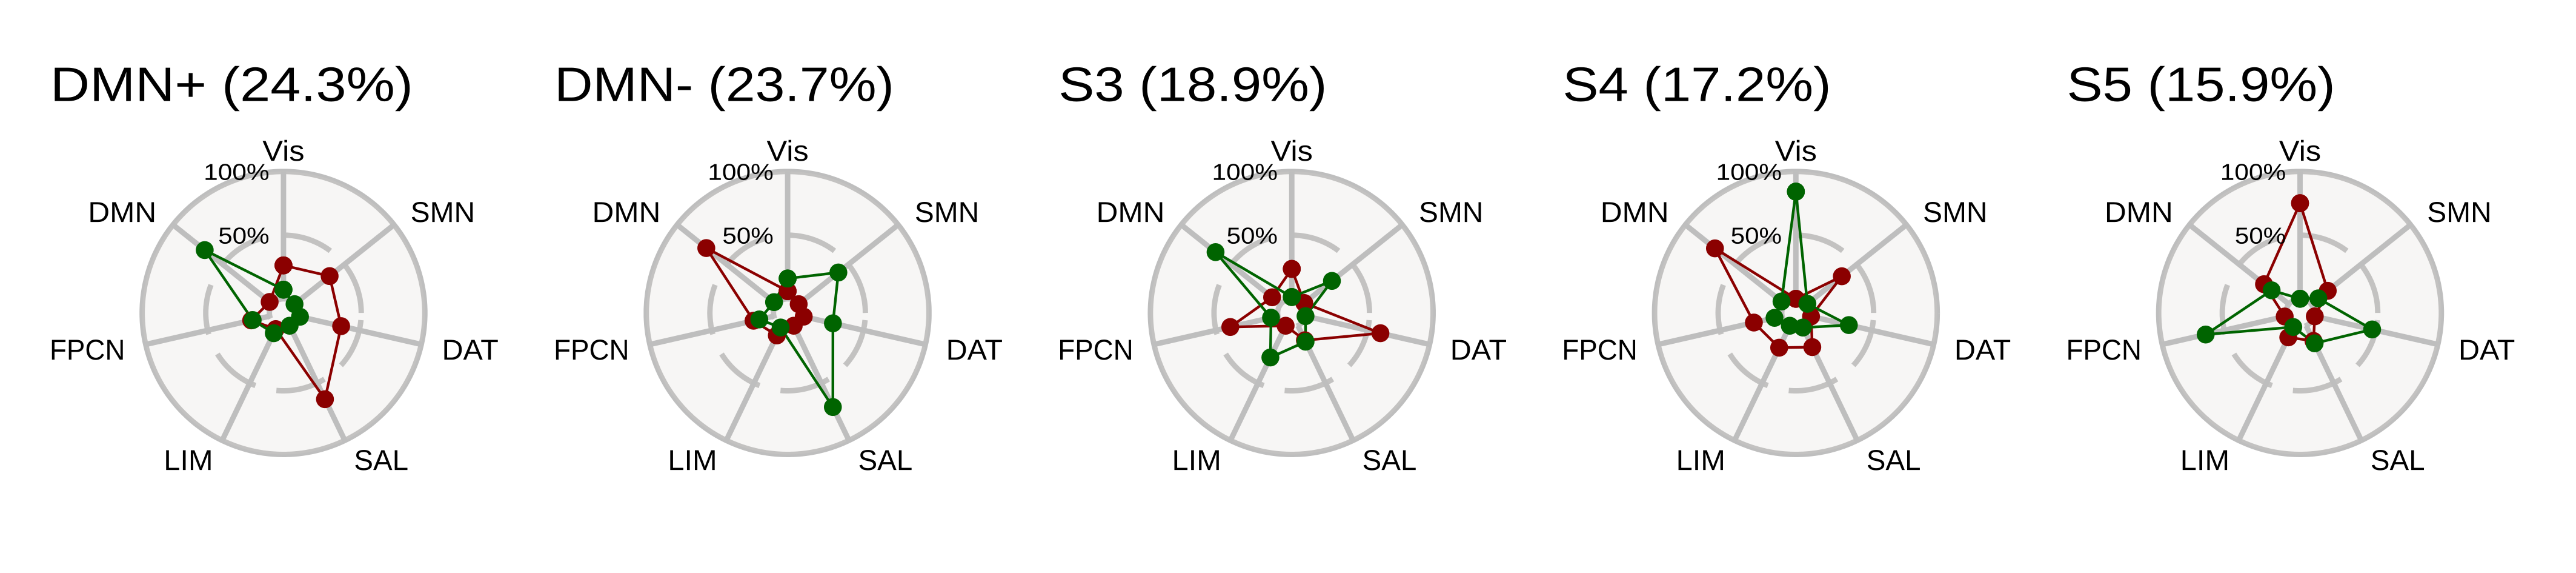
\includegraphics[width=\linewidth]{./../analysis/derivatives/Figures/spiderplot_36p~schaefer400x7.png}
    %\caption{Spider400}
    %\label{fig:spider400}
    %\end{subfigure}
    % \begin{subfigure}{1.0\textwidth}
    % 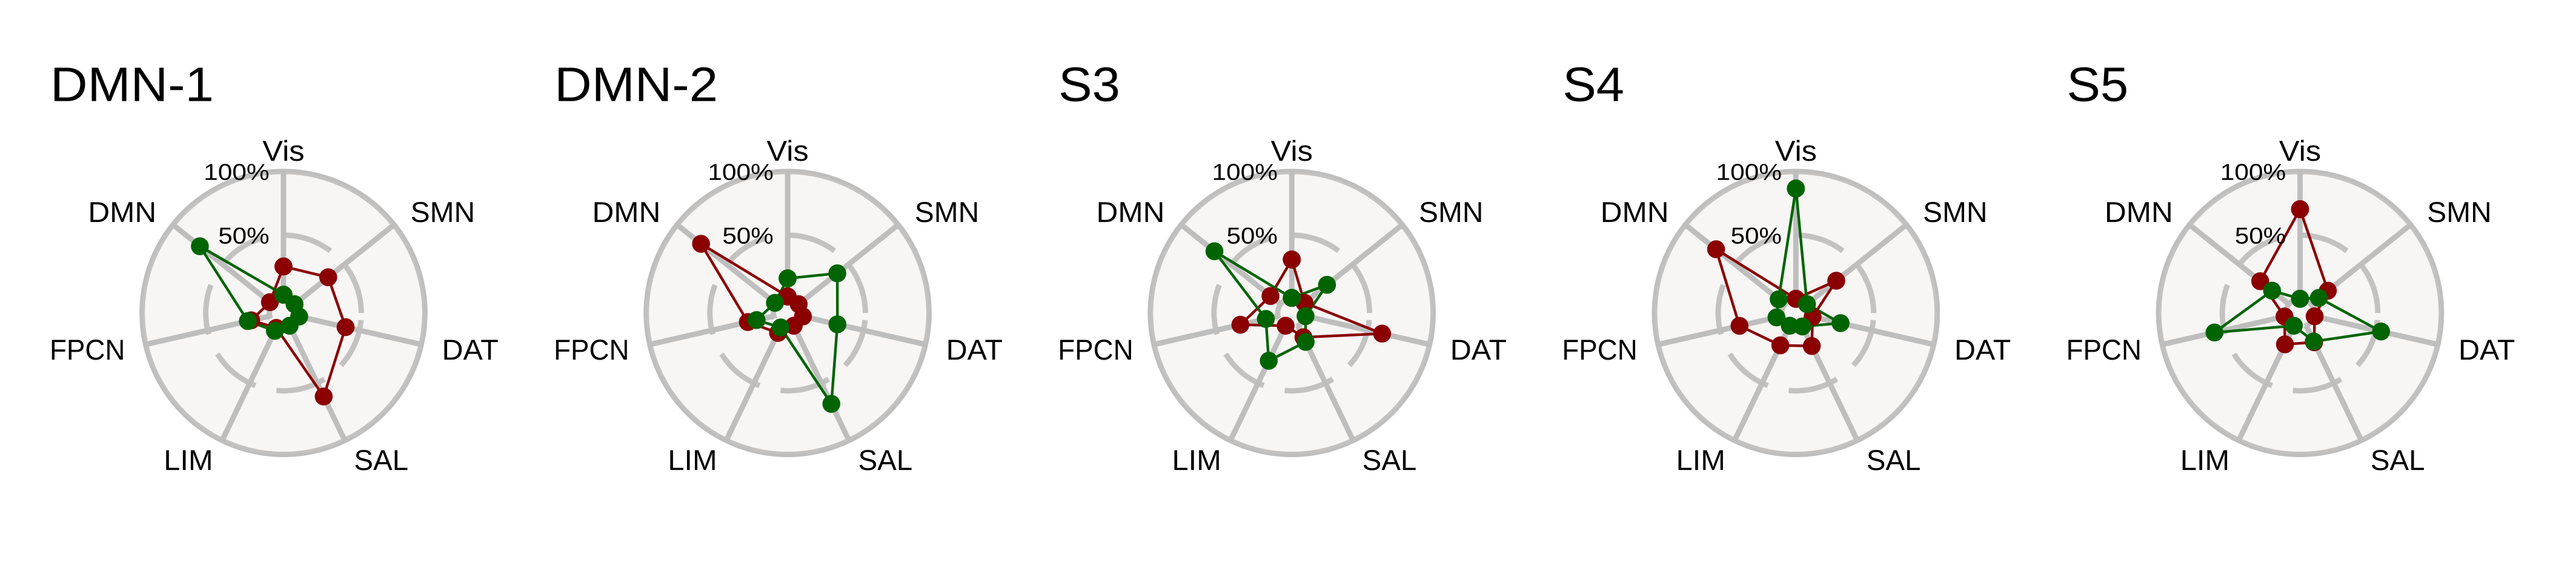
\includegraphics[width=\linewidth]{./../analysis/derivatives/Figures/spiderplot_36p~schaefer200x7.png}
    % \caption{Spider200}
    % \label{fig:spider200}
    % \end{subfigure}
    % \begin{subfigure}{1.0\textwidth}
    %     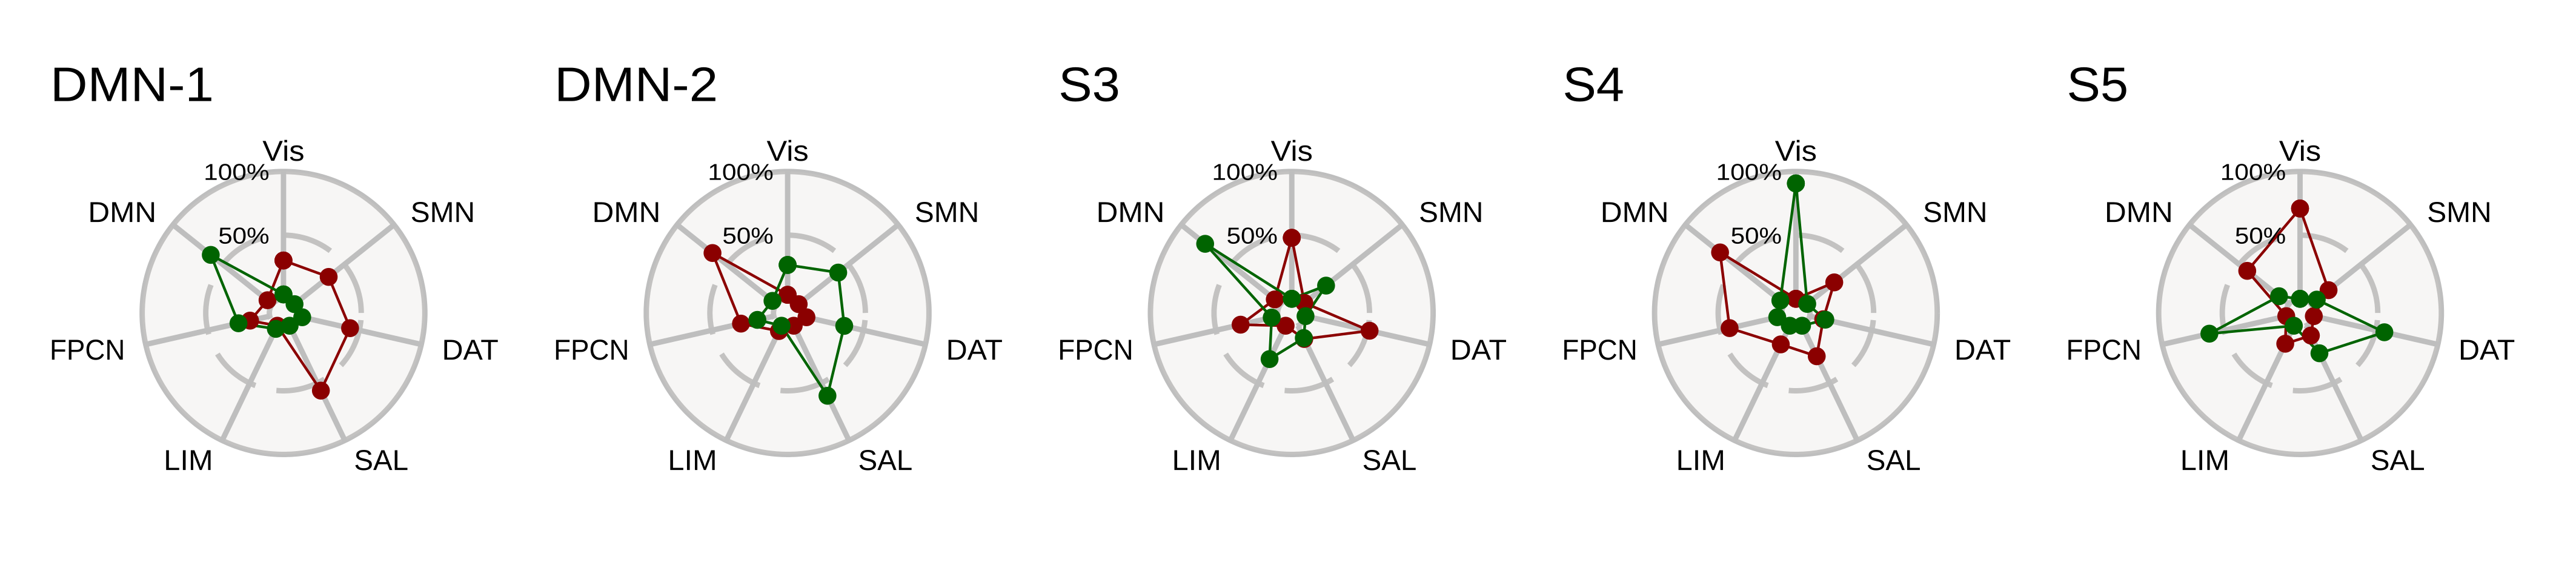
\includegraphics[width=\linewidth]{./../analysis/derivatives/Figures/spiderplot_36p~schaefer100x7.png}
    %     \caption{Spider200}
    %     \label{fig:spider100}
    %     \end{subfigure}
    \mycaption{Connectivity profiles of brain states}{[\textbf{Top}] Centroids of each identified brain state visualized in brain space. Note the individual color scales. [\textbf{Bottom}] Cosine similarity between centroids of brain states and signed indicator vectors corresponding to activation (green) and suppression (red) of each of seven predefined large-scale functional brain networks \citep{Yeo2011-qg}. 
    
    States are ordered by mean fractional occupancy across N=1651 independent participants, indicated by parenthetical percentages. Two high-occupancy states are characterized by activation or suppression of the DMN, the remaining three low-occupancy states (S3--5) were not used in the present study. Note that mean FO values are similar, but not identical, to median FO values reported in \Cref{tab:fracocc}.}
    \label{fig:spider}
\end{figure}


\subsubsection{Association with other cognitive domains}
Associations between the time spent in high-occupancy DMN-related brain states and cognitive measures beyond TMT-B are shown in \Cref{fig:FOvsCOG}.

\begin{figure}
    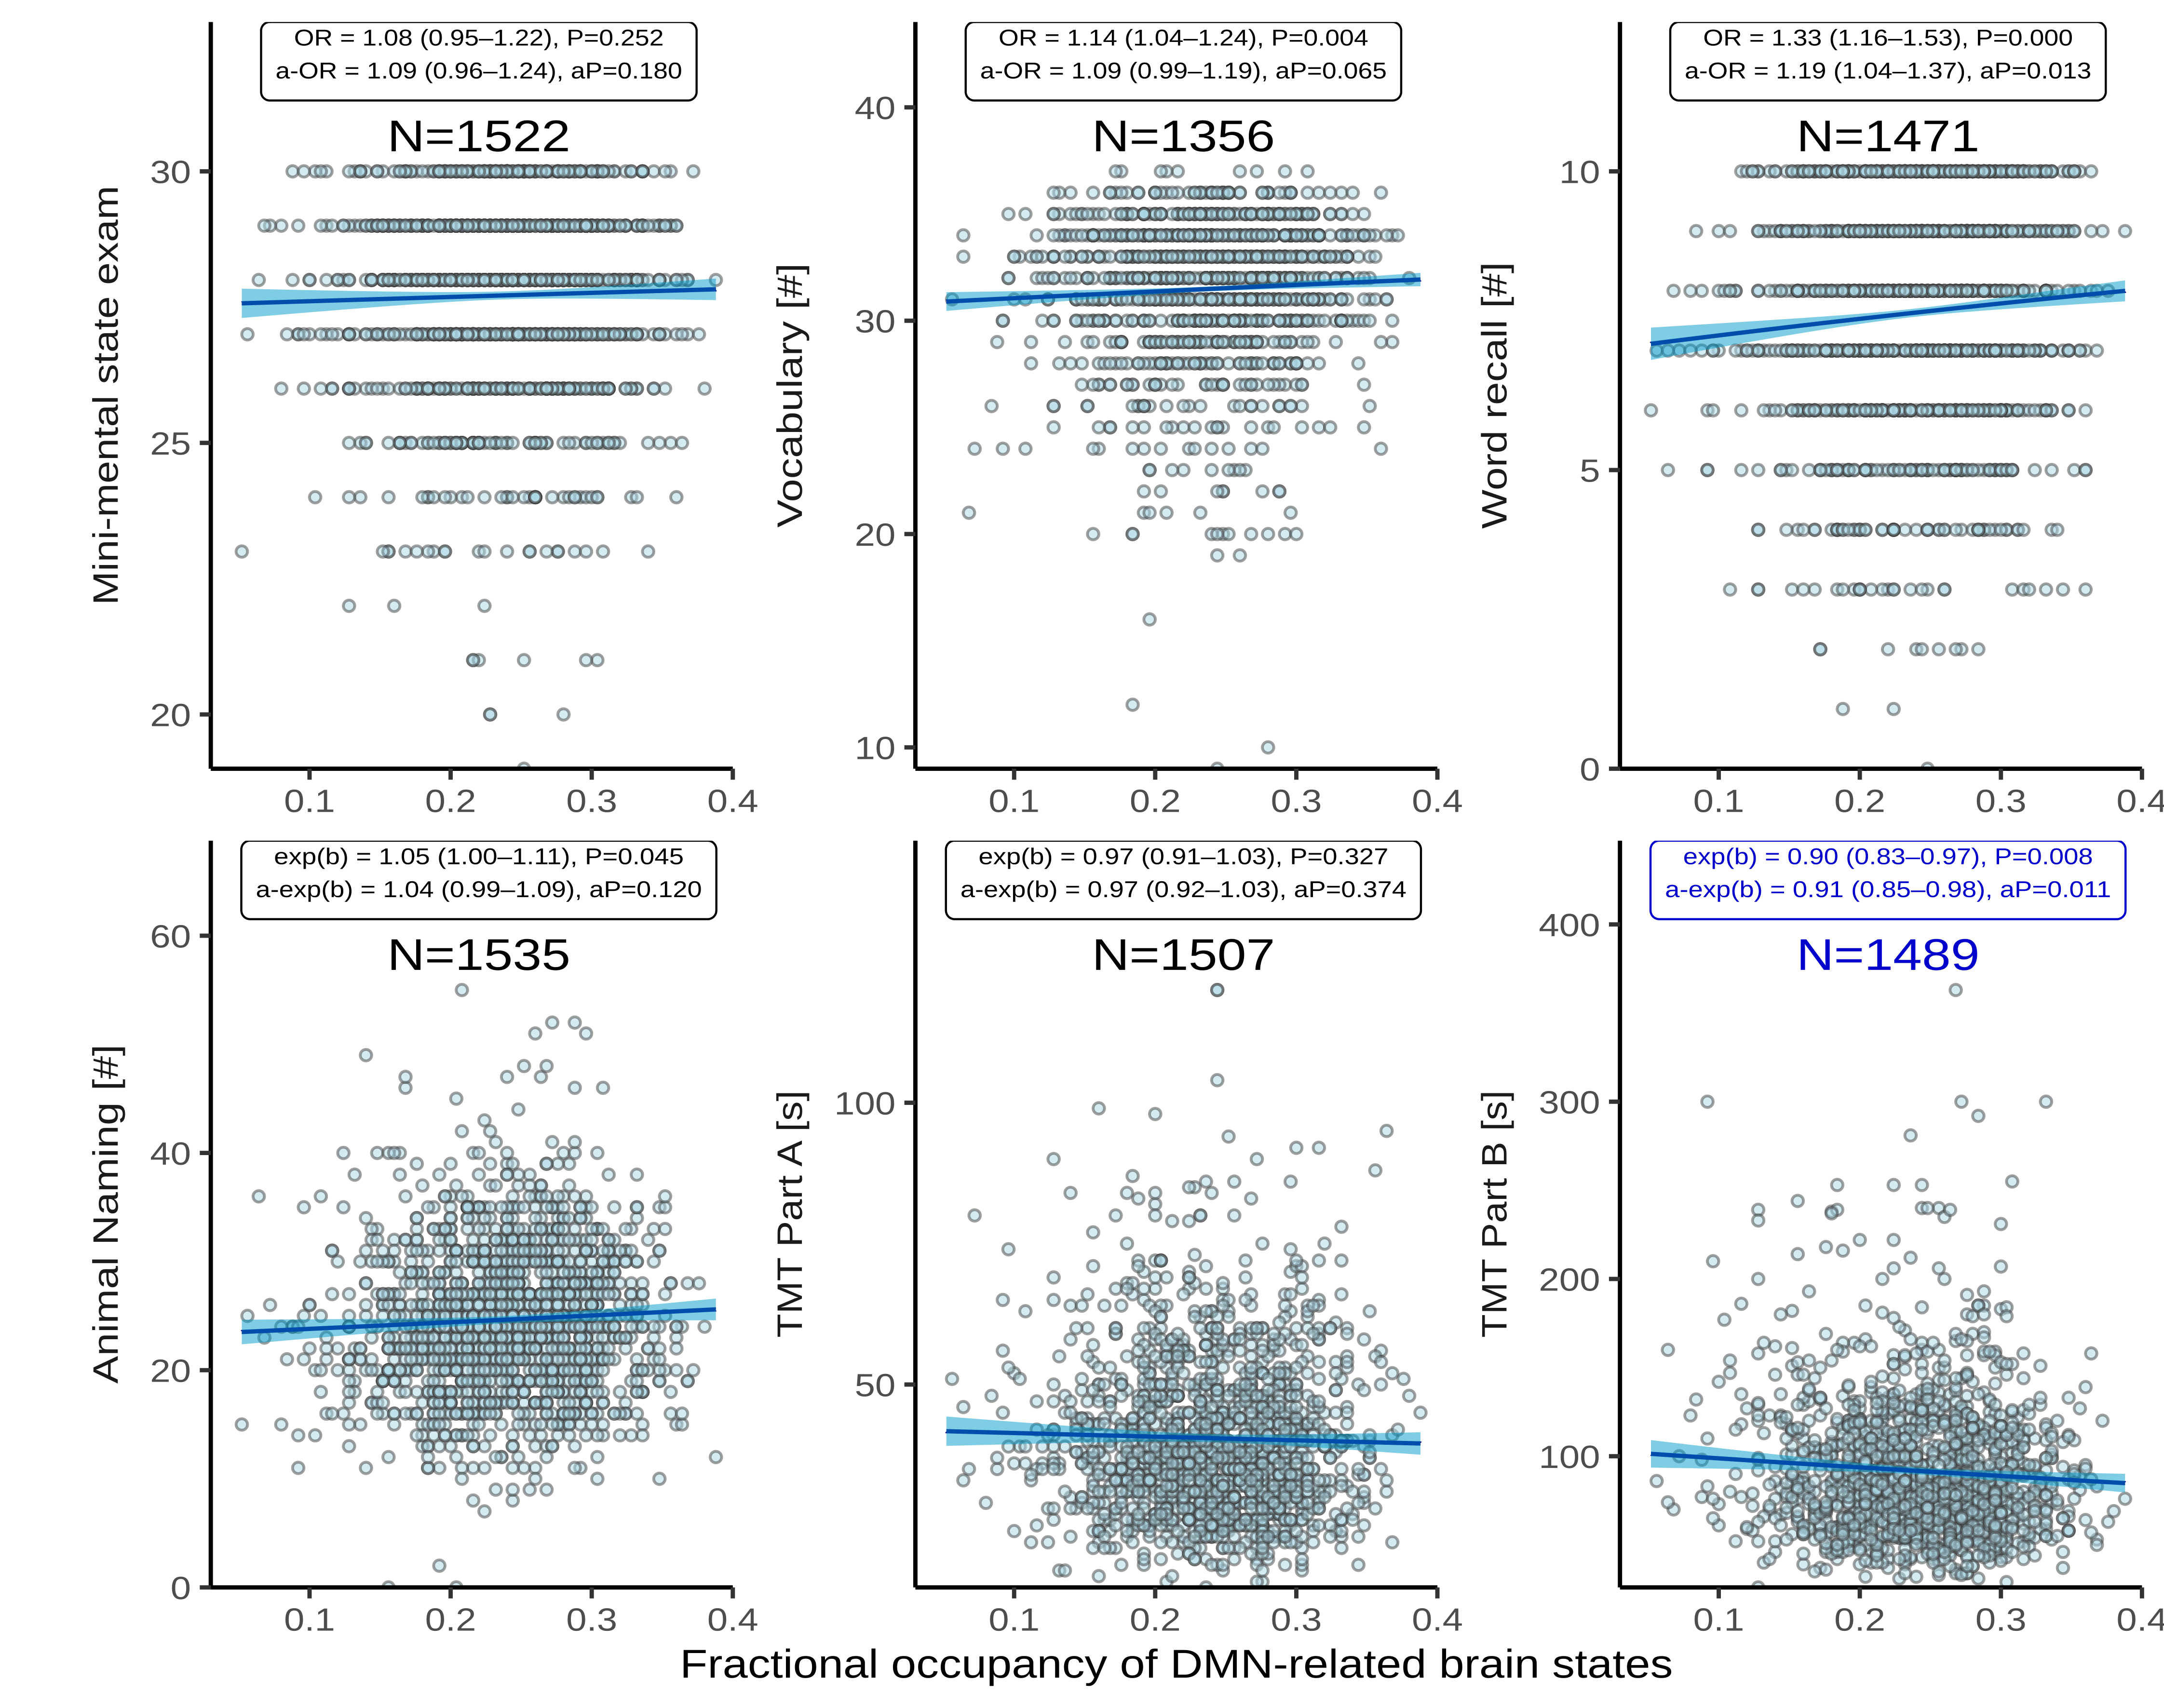
\includegraphics[width=\linewidth]{./../analysis/derivatives/Figures/Fig_FOvsCOG.png}
    \mycaption{Association between time spent in high-occupancy DMN-related brain states and cognitive measures}{Point estimates (black line) and 95\%-confidence region (light blue ribbon) of the conditional mean cognitive measures are obtained from unadjusted binomial (top row: Mini-Mental State Examination, Vocabulary, Word List Recall, logit link) and Gamma regression (bottom row: Animal Naming, Trail Making Test [TMT] A/B: log link) modelling. 
    
    Each marker represents one of N independent participants, as indicated. Insets report effect sizes and P-values both with (adjusted [a-]) and without adjustment for the nuisance variables age, sex, WMH volume (coded as in \Cref{fig:mv}), and years of education. Effect sizes were quantified as odds ratios (ORs) (top) or response scale multipliers [exp(b)] (bottom), and correspond to a 20\%-increase in fractional occupancy. Note the different reference change in FO compared to \Cref{tab:hyp2} chosen to adequately represent some of the smaller effect sizes. The bottom right panel highlighted in dark blue reproduces \Cref{fig:hyp2}.}
    \label{fig:FOvsCOG}
\end{figure}


Adjusted for age, sex, WMH load, and years of education, FO in DMN-related states appeared to be associated with better word recall (adjusted OR 1.19, nominal P 0.013), but not with global cognitive functioning (MMSE, adjusted OR 1.09) or vocabulary (aOR 1.09), nor with verbal fluency (animal naming, adjusted $\exp(\beta)$ 1.04), or pure processing speed (TMT-A, adjusted $\exp(\beta)$ 0.97).
\section{Summary and Discussion} \label{discussion}

In this pre-registered cross-sectional study we replicated the key findings of \cite{Schlemm2022-he} in an independent population-based sample of \num{1651} middle-aged to elderly participants of the Hamburg City Health Study.

First, we confirmed that the severity of cerebral small vessel disease is associated with the time spent in high-occupancy brain states, defined by functional MRI.
More precisely, we showed that every 5.1-fold increase in the volume of supratentorial white matter hyperintensities of presumed vascular origin (WMH) was associated with a 0.95-fold reduction in the odds of occupying a brain state characterized by activation or suppression of the default-mode network, at any given time during the resting-state scan.

Second, we confirmed that the time spent in high-occupancy brain states at rest is associated with cognitive performance. 
More precisely, a 5\%-reduction in the fractional occupancy of DMN-related brain states was associated with a \num{1.02}-fold increase in the time to complete part B of the trail making test (TMT).

In a pre-planned multiverse analysis, findings relating to our primary and, to a lesser extent, secondary hypotheses were robust with respect to variations in brain parcellations and confound regression strategies. Inconsistent results were found with the Desikan--Killiany parcellation, likely reflecting the notion that the spatial resolution and functional specificity of this coarse, structurally defined atlas are inadequate for analyzing functionally defined brain states.  Across brain parcellations, effect sizes  were smaller with the ICA-AROMA confound regression strategy and failed to reach nominal statistical significance. This might be due to a relatively large residual motion component in measures of dynamical functional Connectivity after de-noising with ICA-AROMA, as described previously \citep{lydon2019evaluation}.

We also confirmed across several brain parcellation resolutions that high-occupancy states at rest are characterized by either activation or suppression of the default mode network, reflecting its role as the predominant task-negative brain network.

In unplanned, exploratory analyses, we described the association between brain state dynamics and cognitive measures other than executive function and processing speed and reported a strong, preliminary association between time spent in high-occupancy states and delayed word recall.

We further explored, and report in the Supplementary appendix, the effect of motion; results relating to our primary and, to a lesser extent, secondary, hypotheses were robust to additional, unplanned adjustments for DVARS, RMSD, and mean framewise displacement.

The presented results provide robust evidence for a behaviorally relevant association between cerebral small vessel disease and functional brain network dedifferentiation. 

Further research is required to replicate our findings in different populations, such as those affected more severely by cSVD or cognitive impairment, or being studied using different imaging protocols, to determine the generalizability of our findings with respect to varying operationalizations of the notions of cSVD, brain state, and cognition, and to understand the mechanisms underlying the reported associations.


\subsection{Acknowledgment}
This preprint was created using the LaPreprint template (\url{https://github.com/roaldarbol/lapreprint}) by Mikkel Roald-Arb\o l \textsuperscript{\orcidlink{0000-0002-9998-0058}}.

\subsection{Disclosure}
The authors of this article declare that they have no financial conflict of interest with the content of this article.

%\subsection{Author contributions}
% According to https://journals.biologists.com/jeb/pages/author-contributions

\printbibliography

% DON'T EDIT. If "endfloat" option is enabled all floats appear before appendices
\if@endfloat\clearpage\processdelayedfloats\clearpage\fi 


%%%%%%%%%%%%%%%%%%%%%%%%%%%%%%%%%%%%%%%%%%%%%%%%%%%%%%%%%%%%
%%% SUPPLEMENTARY MATERIAL / APPENDICES
%%%%%%%%%%%%%%%%%%%%%%%%%%%%%%%%%%%%%%%%%%%%%%%%%%%%%%%%%%%%
%% Sadly, we can't use floats in the appendix boxes. So they don't "float", but use \captionof{figure}{...} and \captionof{table}{...} to get them properly caption.
% \begin{appendix}

% \begin{appendixbox}\label{app:ttt}
%     \renewcommand\cellset{\renewcommand\arraystretch{0.5}%
    \setlength\extrarowheight{0pt}}
\begin{table}[bt]
    \scriptsize
    \begin{fullwidth}
        \begin{threeparttable}
            \begin{spacing}{0.8}\centering
                \begin{tabularx}{1.3\textwidth}{p{.2\linewidth} p{.1\linewidth} p{.09\linewidth} p{.15\linewidth} p{.09\linewidth} p{.14\linewidth} p{.08\linewidth}}
                    \toprule
                    Question   & Hypothesis     & Sampling plan     & Analysis plan   & Rationale for deciding the sensitivity of the test & Interpretation given different outcomes & Theory that could be shown wrong by the outcome \\
                    \midrule
                    Is severity of cerebral small disease, quantified by the volume of supratentorial white matter hyperintensities of presumed vascular origin (WMH), associated with time spent in high-occupancy brain states, defined by resting-state functional MRI & 
                    Higher WMH volume is associated with lower average occupancy of the two highest-occupancy brain states. & 
                    Available subjects with clinical and imaging data from the the HCHS \citep{Jagodzinski2020-lx} & 
                    Standardized preprocessing of structural and functional MRI data • automatic quantification of WMH • co-activation pattern analysis • multivariable generalised regression analyses &
                    Tradition &
                    \makecell[tp{\linewidth}]{$P<0.05$ --> rejection of the null hypothesis of no association between cSVD and fractional occupancy;\\ $P>0.05$ --> insufficient evidence to reject the null hypothesis}    &
                    Functional brain dynamics are not related to subcortical ischemic vascular disease.    \\
                    \bottomrule
                \end{tabularx}
            \end{spacing}
            \bigskip
            \caption{Study Design Template}
            \label{tab:SDT}
        \end{threeparttable}
    \end{fullwidth}
\end{table}
% \end{appendixbox}

% \begin{appendixbox}
%     \renewcommand\cellset{\renewcommand\arraystretch{0.5}%
    \setlength\extrarowheight{0pt}}
\begin{table}[bt]
    \begin{threeparttable}
        \begin{subtable}[t]{.75\textwidth}
            \label{tab:parcellations2}
            % Use "S" column identifier to align on decimal point 
            \begin{tabularx}{\textwidth}{l l l}
                \toprule
                \textbf{Name of the atlas}  & \textbf{\#parcels}                                  & \textbf{Reference}          \\
                \midrule
                Desikan--Killiany           & \num{86}                                            & \cite{desikan2006automated} \\
                AAL                         & \num{116}                                           & \cite{tzourio2002automated} \\
                Harvard--Oxford             & \num{112}                                           & \cite{makris2006decreased}  \\
                glasser360                  & \num{360}                                           & \cite{Glasser2016-ia}       \\
                gordon333                   & \num{333}                                           & \cite{Gordon2016-wy}        \\
                power264                    & \num{264}                                           & \cite{Power2011-xf}         \\
                schaefer\{N\}               & \makecell[lt]{\num{100} \\ \num{200}\\ \num{400}}   & \cite{Schaefer2018-bo}      \\
                \bottomrule
            \end{tabularx}
            \begin{tablenotes}
                \item{AAL:} Automatic Anatomical Labelling
            \end{tablenotes}
            \caption{Parcellations}
        \end{subtable}
        \qquad
        \begin{subtable}[t]{.75\textwidth}
            \label{tab:parcellations}
            % Use "S" column identifier to align on decimal point 
            \begin{tabularx}{\textwidth}{l l l}
                \toprule
                \textbf{Design}        & \textbf{Reference}                 \\
                \midrule
                24p                    & \cite{friston1996movement}         \\
                24p + GSR              & \cite{macey2004method}             \\
                36p              & \cite{satterthwaite2013improved}   \\
                36p + spike regression & \cite{cox1996afni}                 \\
                36p + despiking        & \cite{satterthwaite2013improved}   \\
                36p + scrubbing  & \cite{power2014methods}            \\
                aCompCor               & \cite{muschelli2014reduction}      \\
                tCompCor               & \cite{behzadi2007component}        \\
                AROMA                  & \cite{pruim2015ica}                \\
                \bottomrule
            \end{tabularx}
            \begin{tablenotes}
                \item GSR: Global signal regression, AROMA: Automatic Removal of Motion Artifacts
            \end{tablenotes}
            \caption{Confound regression strategies, adapted from \citep{Ciric2017-cl}}
        \end{subtable}
        \makeatletter\def\TPT@hsize{}\makeatletter
    \end{threeparttable}
    \mycaption{Multiverse analysis}{Overview over different brain parcellations and confound regression strategies implemented using xcpEngine \citep{ciric2018mitigating}. A total of $9\times 9=81$ analytical combinations were explored to assess the robustness of our results with respect to these processing choices.}
    \label{tab:multiverse}
\end{table}
% \end{appendixbox}

% \end{appendix}

%%%%%%%%%%%%%%%%%%%%%%%%%%%%%%%%%%%%%%%%%%%%%%%%%%%%%%%%%%%%
%%% ARTICLE END
%%%%%%%%%%%%%%%%%%%%%%%%%%%%%%%%%%%%%%%%%%%%%%%%%%%%%%%%%%%%

\setcounter{figure}{0}
\setcounter{postfigure}{0}

\end{document}
